\documentclass[12pt]{article}
\usepackage{rotating}
\usepackage{amsmath}
\usepackage{graphicx}
\graphicspath{{./Images}}
%\usepackage{subfig}
\usepackage{verbatim}
\usepackage{caption}
\usepackage{subcaption}
\usepackage{setspace}
\usepackage{color}
\usepackage{amsfonts}
\usepackage{amssymb}
\usepackage{float}
%\usepackage{bbm}
\usepackage[authoryear,round]{natbib} 
\usepackage{hyperref}
\usepackage{makecell}
\usepackage[toc,page,header]{appendix}
\usepackage{minitoc}
\hypersetup{
colorlinks=true,
linkcolor=blue,
anchorcolor=blue,
citecolor=blue}
%\hypersetup{hidelinks} % hide the ugly red box in footnote links
\setcounter{MaxMatrixCols}{30}
\providecommand{\U}[1]{\protect\rule{.1in}{.1in}}
\pagestyle{plain}
%\setcitestyle{authoryear,round}
\usepackage[margin=1truein]{geometry}
\newtheorem{theorem}{Theorem}
\newtheorem{acknowledgement}[theorem]{Acknowledgment}
\newtheorem{algorithm}{Algorithm}               
\newtheorem{axiom}{Axiom}
\newtheorem{case}{Case}
\newtheorem{claim}{Claim}
\newtheorem{conclusion}{Conclusion}
\newtheorem{condition}{Condition}
\newtheorem{conjecture}{Conjecture}
\newtheorem{corollary}{Corollary}
\newtheorem{criterion}{Criterion}
\newtheorem{definition}{Definition}
\newtheorem{example}{Example}
\newtheorem{exercise}{Exercise}
\newtheorem{lemma}{Lemma}
\newtheorem{notation}{Notation}
\newtheorem{problem}{Problem}
\newtheorem{proposition}{Proposition}
\newtheorem{remark}{Remark}
\newtheorem{solution}{Solution}
\newtheorem{summary}{Summary}
%\doublespacing
\onehalfspacing
\newenvironment{proof}[1][Proof]{\textbf{#1.} }{\ \rule{0.5em}{0.5em}}
\RequirePackage{threeparttable}
\RequirePackage{booktabs}
\RequirePackage{tabularx}
%\graphicspath{{figure/}}
\makeatletter\let\ExpandableInput\@@input\makeatother
% defines ExpandableInput command which solves the
% problem of having noalign problem in the first line
% of input tables
\def\sym#1{\ifmmode^{#1}\else\(^{#1}\)\fi}  % defines
% the superscripts in tables (significance stars)

\begin{document}
\title{Does Pollution Affect Exports? -- Evidence from China\thanks{Thanks note here...}}
\author{Jie Bai\thanks{Department of Economics, Lingnan University, Hong Kong, E-mail: jiebai@ln.hk} \quad Larry D. Qiu\thanks{Department of Economics, Lingnan University, Hong Kong, E-mail: larryqiu@ln.edu.hk} \quad Junji Xiao\thanks{Department of Economics, Lingnan University, Hong Kong, E-mail: junjixiao@ln.edu.hk.  \copyright\ 2022 Jie Bai, Larry D. Qiu and Junji Xiao. All Rights Reserved. }}
\date{August, 2022}
\maketitle
\thispagestyle{empty}
\begin{abstract}
  Trade is usually an important driving force for rapid economic growth, which is almost always accompanied by deterioration in environment, in developing countries. While most existing studies investigate the impact of trade on environment, this paper is among the first to analyze the reverse effects, that is, whether pollution affects exports and if yes, how, by examining the Chinese export and pollution data over the period of 2000 to 2007. Using $\rm PM_{2.5}$ concentrations estimated by the Aerosol Optical Depth as a proxy for air pollution, we estimate the causal effect of air pollution on the Chinese firms' exports, employing thermal inversion as an instrument variable. Our findings suggest that an 1\% increase in $\rm PM_{2.5}$ leads to an 1.09\% reduction in firm-level exports in China during the sample period. This reduction in exports is mainly attributed to the reduction in exports of continuous exporting firms (intensive margin of exports) and partially attributed to the exporters' entry/exit decisions (extensive margin of exports). The mechanism analysis suggests coexistence of two channels of this effect: First, the air pollution may adversely affect productivity and so reduce exports; second, stringent environmental regulation elevates production costs and so further reduces exports. 
\end{abstract}
\begin{quote}
\emph{Keywords:} Export; Air Pollution; Productivity; Environmental Regulation
\end{quote}
\begin{quote}
\emph{JEL Classification:} 
F14, F18, Q51
\end{quote}

\newpage
\setcounter{page}{1}

\section{Introduction} \label{sec:1}
The rapid economic growth is usually accompanied by deterioration in environment in developing countries such as China. From 1998 to 2007, air quality in China deteriorated a lot. The average $\rm PM_{2.5}$ concentration dramatically increased from 32.32 $\mu g/m^3$ to 49.18 $\mu g/m^3$. The mean concentration exceeds WHO air quality guidelines every year, causing concerns about the balance of environment and economic development.\footnote{For fine particulate matter ($\rm PM_{2.5}$), WHO published guideline values for 5 $\mu g/m^3$ annual mean and 15 $\mu g/m^3$ 24-hour mean. See \url{https://www.who.int/news-room/fact-sheets/detail/ambient-(outdoor)-air-quality-and-health} for more information.} Empirical evidences have shown that severe pollution reduces productivity through influencing health of the people both physically and mentally as health is a very important part of human capital \citep{graff2012impact,chang2016particulate,zhang2018impact,fu2021air,somanathan2021impact,Adhvaryu2022}. In this paper, we ask a different but related question: does pollution influence international trade and how? To answer this question, we focus on China and examine whether a
specific type of air pollution, namely, $\rm PM_{2.5}$ pollutant, affect Chinese firms' exports.

There exists a huge literature on the impacts of trade on environment.\footnote{%
See \cite{cherniwchan2017trade} for the most recent survey of the literature.} However, studies on the impacts of environment on trade are rare, which is what we want to contribute in this paper. One of the biggest challenges in the empirical studies of the trade-environment literature is the endogenous
problem. Estimation of pollution and trade has biases, which results in OLS estimates biased. This problem is more serious in the estimation of the effects of pollution on trade because researchers often find good instrumental variables (IV) for trade to study the pollution effects of trade, such as trade agreements and trade shocks. In this study, we overcome this problem using IV method to examine the causal impact of air pollution on firms' exports and the mechanisms of this impact, using the
county-level annual $\rm PM_{2.5}$ concentrations and firms' productivity data in China. In particular, we follow the literature \citep{fu2021air, khanna2021productivity, chen2022effect} to use both thermal inversion and wind data as IVs for $\rm PM_{2.5}$ concentration.

Our empirical findings suggest that exports decrease as $\rm PM_{2.5}$ levels increase. Specifically, following a 1\% increase in $\rm PM_{2.5}$ concentration, the average exporter decreases its export value by 1.09\%. Air pollution also influences firms' exporting decisions: faced with a 1\% increase in $\rm PM_{2.5}$ concentration, the probability of firms to enter foreign markets decreases by 0.06 percentage points and the probability of exporters to exit foreign markets increases by 0.15 percentage points. The results from estimating the regressions of labor productivity and total factor productivity (TFP)
suggest that air pollution generates detrimental effects on both types of productivity, which echoes with the findings in the previous literature e.g.,\citep{greenstone2012effects,fu2021air,khanna2021productivity}. Also, we find that the negative effect of air pollution on exports only occur to the firms in the regions with specified pollution abatement target, while it is insignificant in the regions without specified pollution control target, suggesting that another working mechanism of the negative effect of air pollution on exports is through regulation costs: Governments in pollution-intensive regions impose more stringent control on pollution, raising the costs of production and so undermining the firms' comparative advantage of exports. This provides additional evidence supporting the previous studies on how environmental regulations affect individual
exporters \citep{cherniwchan2022international}.

This paper is related to the literature on international trade and environment. Several review articles of this literature are available including \cite{cherniwchan2017trade} and \cite{cherniwchan2022international} as the most recent ones. Almost all papers focus on how international trade affect pollution largely through the lens of comparative advantage. Countries that have comparative advantages in pollution-intensive industries with lax
environment policies would export polluting good, so-called pollution haven hypothesis \citep{copeland1994north,taylor2005unbundling}.

Researches on how environmental factors affect international trade are
lacking, with a few exceptions. \cite{jones2010climate} find that one degree
Celsius increase in temperature reduces the growth of the country's exports by 2.0 to 5.7 percentage points significantly for poor countries. \cite{dellink2017international} discuss the potential channels of the environmental effects
through direct impact on transport and distribution chains, and indirect
influences on factors of production. Unlike these papers, we directly
investigate the pollution impact on trade, examine the heterogeneity of this impact in different directions, and identify its potential working mechanisms.  

Our study is also related to a small literature on the impacts of
environmental regulations and policies on various economic outcomes,
especially on productivity and trade. The effects of environmental
regulations on productivity are mixed. \cite{berman2001environmental} find that TFP
rises in air quality regulation regions as abatement investment appear to be
productivity enhancing in the US. \cite{greenstone2012effects} find stricter air
quality regulations are associated with a roughly 2.6 percent decline in TFP
in the US. \cite{he2020watering} find that a water quality regulation campaign in
China significantly reduces upstream polluting firms TFP by more than 24\%
compared to downstream. They link this water quality regulations to
political evaluations. Therefore, local government officials were more incentive to
tighten the water quality standards of upstream of monitor stations.

A few recent papers explore the environmental regulations and their
influences on trade.\footnote{Some papers investigate the effects of environmental regulations on foreign
direct investment \citep{dean2009foreign,cai2016does}.} \cite{hering2014environmental} study the Two Control Zones policy in China and find that exports significantly reduce in targeted cities and sharper fall for
pollution-intensity industries. \cite{shi2018environmental} show that pollution
reduction targets in China's Eleventh Five-Year Plan result in exports fall
in targeted cities. Different from these studies, our paper focuses on the
effects of pollution \textit{per se} on exports.

The rest of the paper is orgnanized as follows. We specify our empirical
strategy in Section~\ref{sec:empirical_strategy}. We describe our data and measurements in Section 3.
We present the main empirical findings in Section 4 and explore the
mechanisms in Section 5. We provide concluding remarks in Section 6.

\section{Empirical Model and Identification} \label{sec:empirical_strategy}
This section presents our empirical methodology of estimating the impact of air pollution on exports. Two stage least squares (TSLS) estimation is applied to solve the potential endogeneity problem with pollution.  
\subsection{Empirical Model}
To investigate the impact of air pollution on exports, we assume exports to be a function of pollution; moreover, we control for the major determinants of exports following previous literature \citep[e.g.,][]{Kunst1989,Bernard2003}. Specifically, the export of firm $i$ in county $c$ at time $t$ is given by,
\begin{equation}
log(Export_{ict})=\beta _{0}+\beta_{1}log(P_{ct}) +\mathbf{X}_{ict}^{^{\prime }}\Gamma +\mathbf{W}%
_{ct}^{^{\prime }}\beta _{w} +\delta _{i}+\lambda
_{t} +\epsilon _{ict}  \label{equ1}
\end{equation}%
where, $log(Export_{ict})$ is the logarithmic volume of exports. $Log(P_{ict})$ is the logarithmic air pollution density. The vector $\mathbf{X}_{ict}^{^{\prime }}$ consists of variables measuring the firm characteristics, including the firm age, size, total capital and productivity. 
The firm productivity is measured by either labor productivity or revenue-based total
factor productivity (TFP). Labor productivity is defined as the ratio of the firm's value added to the firm's employee numbers. We estimate TFP using both Levinsohn-Petrin method \citep{levinsohn2003estimating} and Olley-Pakes method \citep{olley1996dynamics}. These two estimates of TFP are denoted as $TFP_{LP}$ and $TFP_{OP}$, respectively.
TFPs are estimated using the output data at two-digit Chinese Standard Industrial Classification (CSIC), considering heterogeneous productivity across industries. All measures of productivity are in logarithmic form and are deflated by respective price index developed
by \citep{brandt2017wto}. As the previous literature \citep[e.g.,][]{jones2010climate} suggests that weather may also affect exports, we also control for the weather effects on exports using variables in the vector $\mathbf{W}_{ct}^{^{\prime }}$, including temperature, precipitation, humidity, wind speed and sunshine duration. $\lambda _{t}$ is the time fixed effects, capturing the time trends and all other possible time-specific shocks such as annual
socioeconomic cycles that affect exports. $\delta _{i}$ is the firm fixed effects, which is
time-invariant, capturing firm-specific unobservable characteristics contributing to exports. $%
\epsilon _{ict}$ is the error term, which is assumed to be mean zero and independent across firms, allowing within-firm auto correlation. 

% Our outcome variable $Y_{ict}$ are about the intensive margin
% measurement of export: natural logarithm form of the export value of continuing
% exporting firm $i$ in county $c$ and year $t$\footnote{%
% In the way, we only keep export firms that is continuing in exporting from
% the year they started exporting to the last observation year in data.
% Another way to look at intensive margin is keep exporters and observation
% with positive export value, which we show in Appendix A.1.}, and the
% extensive margin of export: the entry \& exit decisions of export of firm $i$
% in county $c$ and year $t$.
One concern with this model identification is the endogeneity problem of pollution: The determinants of exports may affect firms' outputs and so the emission of pollutants, resulting in a correlation between the independent variable $Log(P_{ct})$ and the error term $\epsilon _{ict}$. Intuitively, the increased exports and deteriorated environment could be the simultaneous consequence of positive shocks to production. This endogeneity problem makes ordinary least sqaures (OLS) estimators biased.\footnote{The OLS estimator could suffer from upward or downward bias. For example, high-tech firms may upgrade their production technology over time and adopt energy-saving and environmentally friendly technology. In this scenario, low pollution and high exports are observed, attenuating the negative effects of pollution on exports and so leading to upward bias. In the contrary, less productive firms
may have insufficient funds to upgrade their production technology over
time. In this scenario, OLS estimator generates downward bias. Local
environmental regulations may also bias the OLS estimators. Regions with more exports usually observe faster economic growth at the cost of pollution. In response, the local governments may impose more stringent environmental
regulations, leading to low pollution but high production costs and so low exports \citep{cherniwchan2022environmental,shi2018environmental}; as a consequence, the OLS estimator will also suffer from downward bias.}
\subsection{Identification} \label{sec:identification}
To address this problem, we use instrumental variables (IVs) for $log(P_{ct})$ and apply TSLS estimation to equation~\ref{equ1}. Following the literature \citep{arceo2016does,jans2018economic,sager2019estimating,fu2021air,khanna2021productivity}, we use county-level days of thermal inversion (TI) per annum as IV. In the first stage of the TSLS, we regress the pollution on TI and the other control variables in model~\ref{equ1} and get the fitted value of $Log(P_{ct})$ to be used for the second stage of the model regression. 

TI is a reversal of the normal behaviour of temperature in the troposphere (the region of the atmosphere nearest Earth's surface). Under normal conditions air temperature usually decreases with height. When TI happens, a layer of cool air at the surface of the troposphere is overlain by a layer of warmer air, which acts as a cap on the upward movement of air from the layers below (see
Fig.~\ref{fig:1}). Consequently, convection caused by the heating of air from below is limited to levels below the inversion and so air pollution is trapped close to the ground due to TI. This positive correlation between air pollution and TI is owing to the meteorological factors. 

\begin{center}
  $<$Figure~\ref{fig:1} Here$>$
  \end{center}

There are three typical reasons for
thermal inversion: First, a subsidence inversion occurs when there is
a high pressure system and air from high pressure center in the atmosphere
sinks down to fill the space left as air is blown outward, resulting in a layer
of hot air on a layer of cold. Second, thermal inversion can happen when air
moves horizontally and a warm air layer is squeezed upwards onto the cold
denser air. Third, a radiation inversion happens when air temperature
near ground is cooled down faster than the air above, making the temperature near ground lower than the upper layers.

  Thermal inversion satisfies three conditions for a valid IV: Relevance, exogeneity and exclusion. First, as we discussed above, TI is
  positively correlated with pollution, satisfying the relevance
  condition. The TI is correlated with pollution because the warm layer acts like a roof that traps
  denser cold air containing pollutants near the ground, making it difficult for the pollutants
  to diffuse for short-term. Fig.~\ref{fig:2} shows the relationship between
  TIs and $\rm PM_{2.5}$ concentrations. The top panel shows a strong
  positive correlation between TIs and $\rm PM_{2.5}$ concentrations. The bottom panel shows the trends of TIs and $\rm PM_{2.5}$ over the period of 1998-2007. Even though there is no obvious
  trend of TIs, which suggests that annual thermal inversions is fairly random, air
  pollution trended up over time in China. More importantly, the air pollution is systematically higher in the areas with high TI frequencies than in the areas with low TI frequencies, suggesting a positive correlation between TI occurrence and $\rm PM_{2.5}$ concentrations. Second, no evidence suggests that TI is correlated with exports. It is driven by meteorological factors but not by socioeconomic factors, and so it is not correlated with economic activities such as exports. Lastly, TI satisfies exclusion restriction. As discussed previously, the only channel through which TI may affect exports is pollution. All these features of TI make it a valid and commonly used IV for pollution in the literature \citep{arceo2016does,jans2018economic,sager2019estimating,chen2022effect,khanna2021productivity}.  
% \subsection{IV Approach} \label{sec:2.2}

% The identification requires the $Export_{ict}$ is independent with $\epsilon
% _{ict}$ conditional on control variables. However, the effects of the air
% pollution on export may not be causal, because of export and pollution are
% simultaneous. That is, the increasing of trade corresponding to expanding of
% production companies with deteriorated environment. Absent any effect of
% pollution on exports, higher exports in a county would lead to both higher
% production and worse pollution. In this case, $\hat{\beta _{1}}$ in Eq.(\ref%
% {equ1}) may subject to bias upward. Fixed effects estimators exacerbate
% measurement error, biasing $\hat{\beta _{1}}$ further upward toward to zero.
% The other endogenous problem is omitted variable due to locally time-varying
% changes that lead to either underestimate or overestimate effects of
% pollution on exports in the OLS estimates. For example, counties within more
% high-tech firms may upgrade their production technology over time and
% implement more advanced productive energy-saving \& environmentally friendly
% technology, leading to upward bias. In the contrary, less productive firms
% may have insufficient funds to upgrade their production technology over
% time, leading to a downward bias as technology degrades. Trends in local
% environmental regulations also bias OLS estimates. Regions with more exports
% coincide with faster economic growth impose more stringent environmental
% regulations over time, leading to a downward bias. To identify the
% causality, we apply an instrumental variable approach. The instrumental
% variable is used to predict the $\rm PM_{2.5}$ concentrations across counties but has
% no direct effect on export. The endogenous variable $Log(PM_{2.5})_{ict}$ is
% instrumented by annual days with thermal inversion for each county to
% isolate the causal effect of export on pollution.


% We use the two-stage least squares (TSLS) to estimate: 
% \begin{equation} \label{equ2}
% Y_{ict} = \beta_{0} + \beta_{1} Log(PM_{2.5})_{ict} + \beta_{2}%
% \mathbf{W}_{ict} + \mathbf{X}^{^{\prime }}_{ict} \Gamma + \delta_{i} +
% \lambda_{t} + \epsilon_{ict}
% \end{equation}
% where the fitted value of $Log(PM_{2.5})$ for
% county $c$ in year $t$, is generated by the first-stage regression in the IV
% framework: 
% \begin{equation}  \label{equ3}
% Log(P_{ct}) = \alpha_{0} + \alpha_{1}TI_{ct} + \alpha_{2}\mathbf{W}%
% _{ct} + \mathbf{X}^{^{\prime }}_{ict}\Phi + \delta_{i} + \lambda_{t} + \mu{%
% ct}
% \end{equation}
% where, $TI_{ct}$ is the annual days of thermal inversion for
% county $c$ in year $t$. Standard error is clustered at firm level, but we
% also check the robustness of standard errors at county-year level pattern
% that allows spatial correlation within each county-year.

  \begin{center}
    $<$Figure~\ref{fig:2} Here$>$
    \end{center}

\section{Data and Measurement} \label{sec:3}
\subsection{Pollution Measures and Data}  \label{sec:3.1}
There are different measures for air pollution. The US Environmental Protection Agency has identified six pollutants as ``criteria'' air pollutants, including carbon monoxide, lead, nitrogen oxides, ground-level ozone, particle pollution (often referred to as particulate matter), and sulfur oxides. These pollutants are found to harm human health and the environment. Among these pollutants, the particulate pollutant that is 2.5 microns or smaller in size, or $\rm PM_{2.5}$, is widely used in the literature as an index for air pollution \citep{fu2021air,khanna2021productivity}. Following these studies, we also use the density of $\rm PM_{2.5}$ to measure the air pollution. 

We use the satellite-based $\rm PM_{2.5}$ concentration estimated by \cite{van2021monthly}\footnote{%
    They estimated fine particulate matter ($\rm PM_{2.5}$) by combining Aerosol Optical
    Depth (AOD) retrievals from the NASA MODIS, MISR, and SeaWIFS instruments
    with the GEOS-Chem chemical transport model, and subsequently calibrating to
    global ground-based observations using a Geographically Weighted Regression
    (GWR) at high grid resolution. The Global
    Annual $\rm PM_{2.5}$ Grids data is available on the website of the Atmospheric Composition Analysis Group at Washington University in St. Louis ( \url{https://sites.wustl.edu/acag/datasets/surface-pm2-5/}).} for our analysis. The concentration is available at a spatial resolution of 0.01- by-0.01-degree latitude-longitude grid of the GIS raster (approximately 1.11 kilometers by 1.11 kilometers). To our best knowledge, this is the finest resolution for the concentration data. This satellite-based data has a few advantages 
   over ground-based official source of pollution data. First, the satellite-based
    $\rm PM_{2.5}$ cover all counties, the smallest administrative unit in China, and are available from 1998, whereas the official $\rm PM_{2.5}$ data are only available for large cities since
    2012.\footnote{On February 29 2012, the State Council of China firstly agreed to issue the
    newly revised Ambient Air Quality Standards. The new standard adds monitoring indicators for fine particulate matter ($\rm PM_{2.5}$) and ozone ($O_{3}$%
    ). Therefore, the official data of $\rm PM_{2.5}$ concentration was not available until then.} Second, official air quality data may be potentially manipulated by
    local officials before publication \citep{ghanem2014effortless,andrews2008inconsistencies},  because local environmental quality
has become a vital criterion for government officials’ promotion evaluation since 2006 and particularly after 2015 \citep{Fan2022}. 

    The grid $\rm PM_{2.5}$ concentration is aggregated to the county level. For each county, the annual $\rm PM_{2.5}$ concentration is calculated by taking the mean of values of all grid cells spanning the county. Figure~\ref{fig:3} shows the county-level average concentration of $\rm PM_{2.5}$
over the period of 1998 to 2007 in China. There is substantial spatial
variation in $\rm PM_{2.5}$ concentrations across counties, ranging from
 1.33 $\mu g/m^{3}$ to 97.57 $\mu
g/m^{3}$. The northeastern and eastern regions and southern Xinjiang areas, an autonomous territory in northwest China, suffer from more severe air pollution. As most of these areas also observe higher economic growth rates than the other inland areas during the same period,\footnote{The economic growth in northeast of China and Xinjiang is lower than the other areas. Their air pollution mainly stems from coal-fired power plants. Moreover, coal mining, vehicle emissions, industrial factories, and underground coal fires also contribute to its heavy air pollution. For example, Xinjiang provides the rest of China with 40.6 percent of its coal supply. Its capital city, Urumqi, is the number one coal-consuming city in China.} this suggests that economy may have developed at the cost of environment in China. The heterogeneity in air pollution could be attributed to the difference in physiographic and meteorological conditions across regions. Moreover, the regional socioeconomic factor such as economic activities and environmental policies may also play a significant role in determining the air pollution: Considerable variation in air pollution remains even if we control for the county-fixed effects.

\begin{center}
  $<$Figure~\ref{fig:3} Here$>$
  \end{center}

  \subsection{Thermal Inversions and Weather Controls}\label{sec:data_TI}
The thermal inversion is defined as the phenomenon of air temperature at the
near ground second layer being higher than the first layer. To measure TIs, we exploit the vertical temperature data from
  NASA Modern-Era Retrospective Analysis for Research and Applications (Version 2, or MERRA-2)\footnote{%
  This dataset is titled M2I6NPANA and available at %
  \url{https://disc.gsfc.nasa.gov/datasets/M2I6NPANA_5.12.4/summary}.}. This
  data set provides 6-hour air temperature at 42 atmospheric layers at a grid level of
  0.5%
  %TCIMACRO{\U{b0} }%
  %BeginExpansion
  ${{}^\circ}$
  %EndExpansion
  by 0.625%
  %TCIMACRO{\U{b0} }%
  %BeginExpansion
  ${{}^\circ}$
  %EndExpansion
  (about 45km by 55km in terms of distance). For each grid cell, we calculate the air temperature
changes from the ground atmospheric layer (in the surface measure conditions of
1000 Hectopascal pressure unit (hPa), which is around 110 meters above sea level) to the second atmospheric layer close to ground (in the measure conditions of 975 hPa, approximately 320 m
above sea level). In normal conditions, the temperature decreases with
altitude and hence the temperature difference between these two layers is supposed to be
negative. If this temperature difference is positive, it is counted as an occurrence of TI. 
Formally, We index the atmospherical layers, corresponding to different pressure levels,\footnote{In some cases, we observe missing temperatures at
lower pressure levels because the altitude of the land surface is high in
that grid. Therefore, we label the atmospherical layers relative to the surface, rather than using the uniform pressure levels. As a result, $l = 1$ is always corresponding to the lowest
pressure level above the surface.} by $l = \{1,2,3,...,42\}$, with $l
= 1$ representing the ground layer, and denote the temperature at layer $l$ to be $T_l$. Then, TI is measured by an indicator function $TI =
I\{T_{l=2} - T_{l=1} > 0 \}$. 
We calculate the number of days with TIs occurrence for each grid cell over a year. Then, we aggregate the grid level TIs to the county average using the cell areas spanning the county as weights. We also calculate air temperature
differences between the ground and third-close-to-ground (the 950hPa layer,
which is around 540m above sea level) layers for robustness check.

The station-level daily weather indicators are obtained from National
Meteorological Information Center of China.\footnote{The dataset is provided by National Tibetan Plateau Data Center \url{(http://data.tpdc.ac.cn)} It contains the daily basic meteorological
variables including air temperature, precipitation,
relative humidity, wind direction and speed, sunshine duration
and barometric pressure, collected from 699 national meteorological stations in China
since year 1951 \citep{Dailymeteorologicaldataset}}. We use
Inverse-Distance-Weighting (IDW) method to convert the station-level observations into county-level data, assigning lower weights to the stations further away from the
county center. Taking into account the nonlinear effects of weather as proposed by \citep{deschenes2017defensive}, we divide the sample distribution of temperature into twenty equal-size quantiles and then count the frequency of the daily temperature (the number of days) falling in these quantiles for each county each year. In this way, we generate a twenty-dimensional vector recording the frequency distribution of the county's temperature. This vector of temperature distribution is finally used as the control variables in our regression. Also, we have the squared terms of precipitation, humidity, wind speed, and sunshine duration as weather controls. 

\subsection{Firm-level Data} \label{sec:data_firm}
The firm characteristics are collected from the Annual Survey of Industrial Firms (ASIF) by China's National Bureau of Statistics (NBS). This dataset covers all firms with annual sales
above RMB 5 million in China from 1998 to 2013. In total, there are over 1.4 million observations for around 430 thousand firms over all provinces in
China. Following the literature \citep[e.g.,][]{fu2021trans}, we use the firms in the manufacturing sector for empirical analysis. 

The ASIF data provide detailed information on the firms' balance sheet, such as gross output, value added,
employment, capital, intermediate inputs and ownership. 
To address the potential data input errors, we drop the abnormal observations that violate the following Generally Accepted Accounting Principles (GAAP): (1) liquid assets are greater than total assets; (2)
total fixed assets are greater than total assets; (3) the net value of fixed
assets is greater than total assets; (4) current depreciation is greater
than accumulated depreciation. Furthermore, we also drop the observations for firms with obviously incorrect and missing 
establishment time (e.g., later than 2007 or earlier than 1900) and the observations
with missing or negative values for any one of the variables including output, value added, employment or capital following \cite{cai2009competition,yu2015processing}. We also drop
firms with employees smaller than 8 following the previous research \citep{brandt2012creative}. Finally, our data set consists of 1,722,982 firm-year observations for 474,300 unique firms. Using the firms' accounting information, we derive variables for our analysis including firm age, which is defined as the number of years from the firm's establishment up to the time of the survey, 
firm size, which is defined as the number of employees, and the capital,
which is the real value of net fixed assets. In our econometric analysis, all these variables are in logarithmic forms. 

The export data comes from the Custom transaction database, which is available from China's General Administration of
Customs(GAC). The dataset provides firm-level import and export information of value and quantity
at HS six-digit code level. We aggregate this dataset to
annual frequency to merge with the ASIF data by using the same method as %
\citep{yu2015processing}. In our sample, there are around 17\% to
23\% firms exporting over years.

\subsection{Summary statistics and stylized facts} \label{sec:data_summary}
This section presents some patterns and stylized facts of the key variables in our sample. Figure~\ref{fig:4} exhibits the patterns of air pollution and exports. Panel~\ref{fig:fig_a} presents the time trends of the county-level average of logarithmic annual exports of manufacturing firms in each county and the average of logarithmic annual $\rm PM_{2.5}$ of each county over years, while Panel~\ref{fig:fig_b} presents the average of logarithmic annual exports and $\rm PM_{2.5}$ over years by counties. Although both average exports and pollution fellow the upward trends from 2000 to 2007 (Panel~\ref{fig:fig_a}), there is a clear negative correlation between $\rm PM_{2.5}$ and exports at county-level (Panel~\ref{fig:fig_b}). This stylized fact provides some preliminary evidence suggesting that the exports could be lower in counties of higher $\rm PM_{2.5}$ concentrations. However, we cannot exclude the possibility that some confounding factors may affect these two variables in opposite way and cause their negative correlation across counties. In the subsequent sections, therefore, we will employ more rigorous analysis to control for such confounding factors and investigate the causal relationship between air pollution and exports. 

Table~\ref{tab:var_definition} and \ref{tab:stat} presents the brief description and the sample statistics of these variables. The upper panel lists the key variables of the firms with continuous positive exports, while the lower panel shows the summary statistics of air pollution measured by $\rm PM_{2.5}$ and annual days of thermal inversions at the county level. This sample covers 1908 counties, which is accounted for around 67\% of the total number of counties in China (2864); and, it covers 96\% of all the cities (321 out of 333 cities) and 91\% of all the provinces in China\footnote{Counties without export records are excluded from our sample.}. On average, there are 19 exporters per county for each year. 

\begin{center}
  $<$Figure~\ref{fig:4} Here$>$
  \end{center}

\begin{center}
  $<$Table~\ref{tab:var_definition} \& \ref{tab:stat} Here$>$
  \end{center}

\section{Empirical Results} \label{sec:4}

This section discusses the estimation results of regression model~\ref{equ1}. We first examine the impact of air pollution on the intensive margin of exports using the results from the sample of firms with continuous exports. Then, we analyze the effects of air pollution on the firms' entry and exit decisions on exports. 

\subsection{Effects of Air Pollution on Extensive Margins of Exports} \label{sec:4.1}

In this section, we investigate the effects of air pollution on the intensive
margin of exports, which is defined as the export value from continuous exporting firms that have exports in
the previous year. 

The estimation results are reported in Table~\ref{tab:main_results}.
Table~\ref{tab:main_results} reports both estimates from OLS and TSLS
regressions. The OLS results suggest that exports are negatively correlated with $\rm PM_{2.5}$ (column 1), and this conclusion still remains even after controlling for the firm characteristics (column 2). However, due to the endogeneity problem of $log(PM_{2.5})$, the estimates from OLS regression are biased.
TSLS is applied, employing TI as IV for $\rm PM_{2.5}$, to address the endogeneity problem. The results from TSLS suggest that the coefficient of $log(PM_{2.5})$ is overestimated by OLS regression. Intuitively, this is because air pollution is positively
correlated with exports: More exports and air pollution both could be the consequence of more production; therefore, when the production is high due to
certain factors that are not controlled directly (omitted variables that
included in the error term), these factors also drive up air pollution,
which partially offsets the negative effect of air pollution on exports,
rendering the coefficient overestimated (or attenuated). 

The upper panel of Table~\ref{tab:main_results} in columns (3) and (4) shows the coefficients of TI in the first stage estimation of $log(PM_{2.5})$, which suggests that $log(PM_{2.5})$ increases as the frequency of TI increases. This positive relationship is intuitive based on our discussion on the validity of TI as an IV for$log(PM_{2.5})$ in section~\ref{sec:empirical_strategy}: TI traps air pollution, lifting the concentration of $\rm PM_{2.5}$. After being instrumented, the variation in the fitted value of  $log(PM_{2.5})$ in the second stage regression of exports becomes independent of production activities, and so the estimation bias is corrected. The
Kleibergen-Paap (KP) Wald rk F-statistic \citep{kleibergen2006generalized} for
weak identification test is much larger than the 10\% critical value (16.38) of Stock-Yogo weak ID test \citep{stock2005asymptotic}, suggesting that thermal inversions is strong
instrument variable.
As the TSLS can address the concerns of endogeneity problem with the OLS regression, we explain our findings using results from TSL hereafter.  

The lower panel of Columns (3) and (4) report results of TSLS
estimates of regression~\ref{equ1}. Additional to the fixed effects controlled in column (3), column (4) also controls for the firm characteristics, such as productivity, age size and capital. The coefficients of $log(PM_{2.5})$ in both columns suggest that air pollution will reduce exports. Moreover, the magnitude of the coefficient of $log(PM_{2.5})$ is slightly higher after controlling for the firm characteristics. On the one hand, these results imply that air pollution may affect exports partially through the channel of affecting firms' productivities, as suggested by the literature \citep{fu2021air}, or affecting firms' investment decisions. More importantly, on the other hand, these results mean that pollution may affect exports through unknown channels other than the well documented productivity channel \cite{fu2021air,khanna2021productivity}. Our results suggest that an one percent increase in $\rm PM_{2.5}$ will lead to a 1.09 percent drop in exports for these firms with continuous exports. This is a remarkable magnitude, considering the average annual growth rate of 18.1\% for exports in China over the sample period. 
We will investigate the working mechanism of the impact of air pollution on exports in section~\ref{sec:mechanism}.    

\begin{center}
  $<$Table~\ref{tab:main_results} Here$>$
  \end{center}

We also check the robustness of our results to the sample selection by using the sample of exporting firms with positive export values. In this case, some firms' exports could be discontinued temporarily for some years. The estimation results are presented in Appendix~\ref{sec:A.1}. Basically, the magnitude of the $log(PM_{2.5})$ coefficients becomes larger, compared with those in Table~\ref{tab:main_results}, when we allow temporary discontinuity of exports. Intuitively, temporary discontinuity \emph{per se} is a strategy of firms in response to elevated air pollution; therefore, the impact of air pollution could be larger in this case compared with the case using the sample of continuous exports for analysis.

The negative effects of air pollution on exports may also be attributed to the mechanisms other than changes of intensive margin. They can also result from less entry to or more exits from exporting sector. Decreases in exports due to these two reasons are defined as extensive margin changes in this study, which will be analyzed in the following section.
\subsection{Effects of Air Pollution on Extensive Margins of Exports} \label{sec:4.2}
 In this section, we test whether the air pollution would affect the
  firms' decision to enter or exit the export market. We extend our sample to include
  both exporting and non-exporting firms for this purpose. 
  
  A firm is defined as an entrant to the exporting market in a year if the firm reported a positive export value in that year but did not report any exports in the previous year. Similarly, a firm is defined as an exit from the exporting market in a year if the firm stopped exports in that year but reported exports in the previous year. Formally, we use binary variables $Entry$ and $Exit$ to indicate the firms' respective entry and exit decisions and the mathematical definition of these two variables is given by Equation~\ref{equ4} and \ref{equ5} respectively as follows. 
%   Definition of $Entry$ and $Exit$ is in following Eq.(\ref{equ4}) and Eq.(\ref%
%   {equ5}), respectively. An $Entry$ is indicated as 1 if a firm reports no
%   exports in year $t-1$ but started exporting in year $t$. Exit exporters are
%   defined as those that export in year $t-1$ but no exports in year $t$. 
  \begin{equation}  \label{equ4}
  Entry_{it} = \left\{ \begin{aligned} & 1 & if \ export_{t-1} = 0 \ and \
  export_{t} > 0 \\ & 0 & if \ export_{t-1} = 0 \ and \ export_{t} = 0
  \end{aligned} \right.
  \end{equation}
  
  \begin{equation}  \label{equ5}
  Exit_{it} = \left\{ \begin{aligned} & 1 & if \ export_{t-1} = 1 \ and \
  export_{t} = 0 \\ & 0 & if \ export_{t-1} = 1 \ and \ export_{t} > 0
  \end{aligned} \right.
  \end{equation}

  As the definition of entry and exit in a given period requires the information of firms' status in the previous period,  observations of the firms' first year are dropped from the sample. We analyze firms' entry and exit decisions using IV-Probit estimation, in which TI is still applied as an IV for air pollution. Basically, we run OLS regression of the endogenous variable (the air pollution) on instrument variable (TI) and exogenous variables and then save the residuals from the first stage. The second step is to run the probit model of entry and exit on air pollution and the residuals from the first stage, together with the other exogenous variables, to get consistent estimator of air pollution \citep{wooldridge2010econometric}. 
%   Note that in $Entry$ case, exporters that were already
%   exporting in year $t-1$ are not included in the sample; in $Exit$ case,
%   firms that were not exporting in year $t-1$ are not included in the sample. 

 Table~\ref{tab:entry_exit} reports the marginal effects of variables in the probit model for both entry and exit decisions, which are estimated using maximum likelihood estimation. The standard errors are estimated by bootstrap. Columns (1) - (4) report the marginal effects of variables on the probability of entering or exiting export market. Columns (2) and (4) include the firm characteristics other than the key variable of our interest, $log( PM_{2.5})$. Similar to the results from the intensive margin analysis, the air pollution generates negative effects on the extensive margins: An increase of $\rm PM_{2.5}$ concentration reduces the probability for the firms to enter the export sector, while it increases the probability for the firms to exit the export sector. All these estimates are statistically significant at 1\% level. We will explain the reasons in Section~\ref{sec:mechanism}. 

 \begin{center}
  $<$Table~\ref{tab:entry_exit} Here$>$
  \end{center}

\subsection{Robustness Check}
This section checks the robustness of our estimation results using aggregated data and different IVs, respectively. 
 \subsubsection{County-level Aggregate Analysis}
 Since the key regressor of our interest, $log(PM_{2.5})$, the weather controls and even the IV, all are featured with county-level variation only, the impact of air pollution on firm-level exports could be attributed to idiosyncratic shocks that share common trends to all firms. We check the robustness of our results using the county-level average of export values and the proportion of entry/exits as dependent variables for our intensive margin (equation~\ref{equ1}) and extensive margin (a linear counterpart for equation~\ref{equ4}) analysis. Specifically, the dependent variable for intensive margin analysis is the logarithmic average export value of firms in county $c$ of year $t$, while the dependent variable for extensive margin analysis is the proportion of new (or exiting) exporters in county $c$ of year $t$, which is defined as (Number of new (or exiting) exporters / Number of exporters).
 
 Table~\ref{tab:by_county} represents the TSLS estimations results using the county-level aggregate data. Columns (1) and (2) show the results for intensive margin analysis with different model specifications, while columns (3) and (4) show the results for extensive margin analysis. In columns (1) and (2), the coefficients of air pollution are both negative and statistically significant, which is consistent with firm-level results, suggesting that $\rm PM_{2.5}$ has negative effects on exports. Moreover, the magnitude of the coefficients is much larger than that of the firm-level analysis, suggesting that a significant portion of the idiosyncratic shocks to exports could share some comments trends with air pollution. For example, in the areas with severe pollution, pollution regulation could be more stringent, which may generate negative effects on export costs \citep{cherniwchan2022environmental}. Although this negative effects could be heterogeneous across firms, depending on their abatement technology, all firms in the administrative region could share the same trend. Since firm-level characteristics are important to explain the difference in cost changes in response to such regulation, most variation in exports could be explained by firm specific shocks when the firm-level data is employed, but this variation is attributed to the air pollution effects when county-level aggregate data is applied, resulting in a larger coefficient of $\rm PM_{2.5}$.
 
  Columns (3) and (4) report the estimation results from regressions of the number shares of entry and exit firms in the export sector of a county\footnote{Mathematically, the number shares ($S$) of entry ($I$) or exit ($O$) firms in the export sector of county $c$ of year $t$ are defined as $S^x_{ct} = N^x_{ct}/N_{ct}, x = \text{I or O}$, where $N^x_{ct}$ is the number of firms that enter ($x = I$) or exit ($x = O$) county  $c$; and $N_{ct}$ is the number of firms in county $c$ of year $t$.}. The results are also consistent with our analysis using the firm-level data. 
 \begin{center}
  $<$Table~\ref{tab:by_county} Here$>$
  \end{center}

 \subsubsection{Alternative IV: wind direction} \label{sec:5.1.1}

 \section{Heterogeneity} \label{sec:5}
%  \subsection{Heterogenous effects} \label{sec:5.2}
%  For heterogenous effects, we should include (1) High vs. low productivity firms (interaction terms with PM2.5 variable), (2) High and low labor intensity, (3) TCZ vs.non-TCZ

 \subsection{Productivity} \label{sec:5.2.1}
 Productivity is a key determinants of exports, as suggested by the previous literature. The negative effects of air pollution on exports could differ in firms' productivity since firms with different productivity may have different capacity to digest the negative effects of pollution on their exports. To test the heterogeneous effects of air pollution on firms with different productivity, we categorize all firms into two groups: high- and low-productive firms. We use the median of the distribution of firm productivity as the threshold to define a dummy variable of high-productivity (= 1 if a firm's productivity is higher than the median; and 0, otherwise). Then, we add a interaction term between $Log(PM_{2.5})$ and this high-productivity dummy to our main regression (Equation~\ref{equ1}) and then apply TSLS to the firm-level data. 

%  \begin{equation}  \label{eq6}
%   \begin{aligned} Log(Export)_{ict} = \beta_{0} + \beta_{1}Log(PM_{2.5})_{ict} + \beta_{3}Productivity\times
%   Log(PM_{2.5})_{ict} \\ + \beta_{4}\textbf{W}_{ict} + \textbf{X}^{'}_{ict}\Phi +
%   \delta_{i} + \lambda_{t} + \epsilon_{ict} \end{aligned}
%   \end{equation}

%   where \textit{Productivity} is indexed either by its revenue-based TFP or by its apparent labor productivity, all in the logarithm form. 

%   Regarding our predictions on air pollution and heterogeneity, the impact of
% $\rm PM_{2.5}$ concentrations ($\beta _{1}$) is expected to be negative, and $\beta
% _{3}$, the coefficient on the interaction term, should be positive: the
% export value elasticity to $\rm PM_{2.5}$ concentrations changes should decrease with
% the firm's performance. 

Table~\ref{tab:hetero_tfp} reports the estimation results. Columns (1) - (3) present results using LP TFP, OP TFP and labor productivity as the measures for firm productivity, respectively. The estimation results are consistent, irrespective of different measures of productivity. The coefficients of all independent variables are similar to those reported in Table~\ref{tab:main_results}. The positive and significant coefficients of the interaction term suggest that air pollution generate weaker effects on firms with higher productivity, implying that more productive firms can better cope with the negative shocks brought by air pollution. 
%In the bottom of these three columns, we report how the total effects of air pollution on exports change with productivity: As the productivity increases from its sample mean to the level of mean plus one standard deviation, the marginal effect of air pollution on exports decreases from -.93 to -.81, when LP TFP is used as the productivity measure. 

  \begin{center}
    $<$Table~\ref{tab:hetero_tfp} Here$>$
    \end{center}

 \subsection{Labor Intensity}  \label{sec:5.2.2}
 A bulk of previous research \citep[e.g.,][]{chang2016particulate,Adhvaryu2022} has documented the detrimental effects of air pollution on workers, and so air pollution may reduce productivity in physically demanding jobs more than it does on the less labor-intensive jobs. This section compares the effects of air pollution on exports across industries with different levels of labor intensity.\footnote{  
 We use industry-level labor intensity instead of firm-level data to alleviate the concerns with the endogeneity of the labor intensity at the firm level, which may arise when firms strategically change their composites of labor intensity in response to air quality shocks.} To investigate the heterogeneous effects of air pollution on exports over industries with different labor intensity, we add an interaction term of labor intensity and $Log(PM_{2.5})$ to regression model~\ref{equ1}. Following the previous literature \citep{dewenter2001state}, labor intensity is measured in two different ways: 1) labors divided by real capital stock; and 2) labors divided by real valued added. The first measure indicates the intensity of labor inputs relative to capital inputs in the production, while the second measure indicates the intensity of labor out of value added. We use a four-digit CSIC code to define an industry. 

%  \begin{equation}
%   \begin{aligned} Log(Export)_{ict} = \beta_{0} + \beta_{1}Log(PM_{2.5})_{ict} +
%   \beta_{2}Labor Intensity_{ict}  + \beta_{3}Labor Intensity\times \\
%   Log(PM_{2.5})_{ict}  + \beta_{4}\textbf{W}_{ict} + \textbf{X}^{'}_{ict}\Phi +
%   \delta_{i} + \lambda_{t} + \epsilon_{ict} \end{aligned}
%   \end{equation}

% where \textit{Labor Intensity} is calculated by different measures, labors divided by real capital stock and labors divided by real valued added \citep{dewenter2001state}. The former indicates the relative use of factors and the latter measures the labor intensity of production. $Labor Intensity_{ict}$ is in the natural logarithm form. Industry labor intensity is calculated at 4-digit level.
\begin{center}
  $<$Table~\ref{tab:hetero_LI} Here$>$
\end{center}

Table~\ref{tab:hetero_LI} reports the estimation results. Columns (1) and (2) report the results using the labor/capital ratio as the measure of labor intensity, while columns (3) and (4) report the results using the labor/value added as the measure of labor intensity. Our findings show that the impact of air pollution on exports is larger for more labor-intensive industries than it is for less labor-intensive industries. The coefficients of the other variables are still very close to those reported in Table~\ref{tab:main_results}, irrespective of the function specifications and the measures of labor intensity. The coefficient of labor intensity is positive, suggesting that the firms in the labor-intensive industry are exporting more than those in less labor-intensive industries. 
 \subsection{Industrial Pollution Intensity} \label{sec:5.2.3}
Industries significantly differ in their pollutant emissions. Manufacturers of chemical product, such as chemical fibers and non-metallic mineral products, generate much more air pollutants than those producing scientific and mathematical instruments. Industries with higher pollution intensity have to pay higher abatement costs to meet the environmental requirements than the industries with lower pollution intensity. Therefore, as air condition deteriorates, the marginal costs due to abatement needs\footnote{Firms have to invest on abatement technology to meet the environmental requirement. This will increase the fixed costs but not the marginal costs. The marginal costs increase because the firms have to go through additional abatement procedure to meet the requirement when the air pollution becomes more severe.} may increase by a larger scale for the firms in the pollution-intensive industries than they do for the firms in the less-pollution-intensive industries, generating heterogeneity in the effects of air pollution on exports.  

We investigate this heterogeneity caused by industrial pollution intensity by estimating model~\ref{equ1} with an additional interaction term of industrial pollution intensity ($PI$) and air pollution $log(PM_{2.5})$. The yearly industrial pollution intensity of pollutant $p$ in sector $k$, $PI^{p}_{kt}$, is defined as the ratio of total emissions of pollutant $p$ in sector $k$ to the total value of output in this sector in year $t$. We use four published pollutants to measure $PI$, including total industrial waste gas, sulfur dioxide($SO_{2}$), soot smoke and suspended particulate matter. The suspended matter includes coarse particles with a diameter of 10 micrometers or less, which covers a broader range of particulate matters including $\rm PM_2.5$.  
We aggregate the $PI$ data to the 2-digit CSIC level from the China Environment Yearbooks (1999-2008) published by the Ministry of Environmental Protection. 

Table~\ref{tab:hetero_PI} reports the results of estimation. $PI^{p}_{kt}$ is in the natural logarithm form. Columns (1)-(4) correspond to different $PI$ measured by by total industrial waste gas, sulfur dioxide($SO_{2}$), soot smoke and suspended particulate matter, respectively. The coefficients of the interaction term of $Log(PI) \times Log(PM_{2.5})$ are all negative and statistically significant, suggesting that the firms in pollution-intensive industries suffer more from the negative impact of air pollution on exports.

\begin{center}
  $<$Table~\ref{tab:hetero_PI} Here$>$
\end{center}

 \subsection{Environmental Regulation} \label{sec:5.2.4}
Environmental regulations will increase abatement costs and such costs may increase in the gap between the policy target and the pollution level, implying that the effects of pollution on exports may differ in environmental regulations. This section intends to test the heterogeneity of pollution effects on exports over places with different levels of environmental regulations. However, it is difficult to directly measure the stringency of regulations as it is usually hard to quantify such regulations. Usually, the standards, targets and the compliance costs of these policies are unclear. Moreover, there are tremendous environmental policies and regulations published nationally or locally, whose effects overlap with each other. 

A national wide environmental policy--Two Control Zones (TCZ), serves as a quasi-natural experiment for analysis of the heterogeneity of the negative effects of air pollution on exports caused by environmental regulations.
In 1998, the State Council tightened the control of acid rain and the emission of sulfur dioxide ($SO_2$) in targeted areas, which are named as TCZ,\footnote{The government approved the establishment of the TCZ through the publication titled ``The Official
Reply of the State Council Concerning Acid Rain Control Areas and $SO_{2}$
Pollution Control Areas''} including 175 prefecture-level cities, accounting for 11.4\% of the nation's
territory, 40.6\% of the population, 62.4\% of GDP, and 58.9\% of total $%
SO_{2}$ emissions in 1995 \citep{hao2001plotting}.  
The government sets clear environmental targets for the cities in TCZ, whereas,  
the rest of 205 cities are not subject to this policy. Although this policy targeted acid rain and sulfur dioxide rather than $\rm PM_2.5$, the establishment of TCZ still indicates the government's concerns with the overall air pollution in the target areas. Therefore, we expect that the firms in TCZ are facing more stringent environmental regulation.

We add an interaction term of a binary variable $TCZ$ (=1 if the county is in TCZ; 0 otherwise) and $PM_{2.5}$ to regression~\ref{equ1}. The estimation results are reported in Table~\ref{tab:hetero_cost}. Column (1) reports the estimation results using the full sample, assuming that the marginal effects of all variables other than air pollution are the same in TCZ and non-TCZ. The coefficient of the interaction term of $TCZ \times log(PM_{2.5})$ is negative and significant at 10\% significance level, suggesting that the air pollution has more adverse effects on exports in TCZ than it does in non-TCZ. However, the coefficient of the independent term of $log(PM_{2.5})$ is insignificant, suggesting that air pollution has no significant effects on exports in non-TCZ areas (where, $TCZ$ = 0). 

Columns (2)-(3) report the results using the sub-samples of observations in TCZ and non-TCZ respectively, without equality constraints on their coefficients. The results are similar to those in column (1). Furthermore, the coefficient of $log(PM_{2.5})$ is negative and statistically significant for the sub-sample in TCZ, while it is insignificant for the sub-sample in non-TCZ. 
\begin{center}
  $<$Table~\ref{tab:hetero_cost} Here$>$
\end{center}

\section{Mechanisms}\label{sec:mechanism}
Previous literature suggest that there could be at least two channels, through which air pollution reduces exports: First, the air pollution may generate immediate and long-lasting detrimental impact on human, reducing productivity at work \citep{chang2016particulate,Adhvaryu2022,khanna2021productivity}. This effect will be more salient for labor-intensive industries, which are the main stream of the Chinese export sector (Table~\ref{tab:hetero_LI}. Previous studies have documented rich evidence on the adverse effects of air pollution on productivity due to lower working efficiency or absence from work caused by health problems \citep{fu2021air,somanathan2021impact}  or migration of high-skilled labor from the pollution-intensive cities \citep{khanna2021productivity}. Second, environmental regulation could be more stringent in more polluted areas as the environmental problem is more aware and so the government faces more abatement pressure, which is passed through to the firms in those areas and converted into their abatement investment, enhancing production costs and harming their comparative advantage in exports \citep{cherniwchan2022environmental,cherniwchan2022international}. This section investigates the working mechanisms of the air pollution on exports, focusing on the productivity and regulation cost channels.    

\subsection{Productivity Channel} \label{sec:6.1}
  To examine whether air pollution reduces exports through the productivity channel, we first study how the firms' productivity changes with air pollution. We employ TSLS estimation to the productivity function (\ref{eq:productivity}), applying TI as IVs to address the endogeneity problem with $Log(PM_{2.5})$.
  \begin{equation}\label{eq:productivity}
    Productivity_{ict} = \beta_{0} + \beta_{1} Log(PM_{2.5})_{ict} + \mathbf{W}_{ict}^{\prime} \beta_{2}%
     + \delta_{i} + \lambda_{t} + \epsilon_{ict}
  \end{equation}
Table~\ref{tab:mechan_tfp} reports the estimation results. Columns (1)-(3) correspond to the regressions of different measures of productivity. Not surprisingly, air pollution generates more adverse effects on labor productivity than on the TFP: one
  percent increase in $\rm PM_{2.5}$ concentrations decreases labor productivity by
  1.51 percent, compared with a decrease of 0.70 or 1.09 in TFP measured by LP or OP methods, respectively. This finding echoes with previous literature \citep{fu2021air,somanathan2021impact,chang2016particulate,Adhvaryu2022}, suggesting that air pollution mainly affect productivity through health channel.  As our findings in Table~\ref{tab:main_results} suggest that exports increase with productivity, it is a natural conclusion that air pollution may affect exports through the productivity channel. 
  
  To examine whether the productivity is the only working channel of air pollution on exports, we run regressions of model~\ref{equ1} controlling for different productivity measures and report the estimation results in Table~\ref{tab:mechan_tfp2}. The main results of our interest are the coefficients of $Log(PM_{2.5})$, which are all negative and significant. This means that even after controlling for the productivity channel, the air pollution still has negative effects on exports, implying that there are still unknown mechanisms behind the causality between air pollution and exports. 
  
  \begin{center}
  $<$Tables~\ref{tab:mechan_tfp} and \ref{tab:mechan_tfp2} Here$>$
  \end{center}
\subsection{Regulation Costs} \label{sec:6.2}
The results in Table~\ref{tab:hetero_cost} have given us some hints on another possible channel of air pollution affecting exports. The estimation results from sub-samples suggest that other than the productivity channel, air pollution also has negative effects on exports in TCZ only, but does not have any effects in non-TCZ. As the main difference between these two zones is the environmental regulation, the effects of air pollution, after partialling out the productivity channel, should be attributed to additional costs caused by environmental regulation, as proposed by \citep{cherniwchan2022environmental}. This finding adds to the literature about the impact of environmental regulations and policies on trade \citep{hering2014environmental,shi2018environmental,cherniwchan2022environmental,berman2001environmental,greenstone2012effects}. 

% Apart from the direct impact on productivity, deteriorative air quality, usually followed by a series of environmental regulations as time goes by, can indirectly influence exports when we treat those environmental regulations as a comparative advantage. The intuition is that
% environmental regulations increase pollution abatement costs of local
% producers which may make them less competitive in foreign markets compared
% with firms that do not face similar regulations. Therefore, the production
% cost of firms within stringent environmental regulations areas is relatively
% higher, thereby deterring exports. The heterogeneity test in TCZ policy infers the potential channel of environmental regulations. Other studies employed DID strategy to verify various environmental regulations and policies on trade flows \citep{hering2014environmental,shi2018environmental,cherniwchan2022environmental}. 
% Stringent regulations imply abatement costs to firms, so that some studies also associate with productivity. i.e.\citep{berman2001environmental,greenstone2012effects}. 

\section{Conclusion} \label{sec:7}
This paper investigates the direct impact of air pollution on exports, using the data of firm-level productivity and county-level air pollution. Recent literature has documented empirical evidence of both the adverse effects of air pollution on productivity \citep{greenstone2012effects,fu2021air,khanna2021productivity} and the positive effects of productivity on exports \citep{Kunst1989,Khandelwal2013}; however, a crucial part in the analysis of the causal effects of air pollution on exports is still missing: no empirical evidence of the direct effects of air pollution on exports has been documents. This paper intends to fill this gap. 

 We explored the effects of $\rm PM_{2.5}$ on both intensive and extensive margins of
  exports. We found that the export values decrease when $\rm PM_{2.5}$ concentrations increase in China during the period of 1998-2007. This adverse of air pollution on exports is more salient for less-productive firms, more labor-intensive firms or more pollution-intensive firms. The mechanism analysis suggests that air pollution may undermine exports through two channels: it hurts the productivity or enhances the production costs when environmental regulation is stringent. 
  
  

\newpage
\small
\bibliographystyle{elsarticle-harv}
\bibliography{pollution}

\newpage
%   \begin{table}[H]\centering
%     \caption{Summary Statistics of Variables in Regression}\label{tab:stat}
%     \resizebox{\textwidth}{!}
%     {
%     \begin{tabular}{l*{4}{c}}
%       \hline\hline
%       &\multicolumn{1}{c}{Description}&\multicolumn{1}{c}{Obs.}&\multicolumn{1}{c}{Mean}&\multicolumn{1}{c}{Std. Dev.}\\             
%       \hline
%       \textit{Firm-level characteristics} &&&&\\
%       Export	&Export value (US Dollars, million) &236,494	&8.1232	&98.8678 \\
%       $TFP_{LP}$	&TFP measured by LP method&236,494	&7.3256	&1.2955 \\
%       $TFP_{OP}$	&TFP measured by OP method&236,494	&3.5074	&1.3503 \\
%       Labor productivity &ln(Value added/No. labors) &236,494	&4.0266	&1.1562 \\
%       Firm Age 	& Years of incorporation of the firm &236,494	& 8.5556 &8.0523\\
%       Firm Size	& Employees of the firm &236,494	&415.0815	&1247.016 \\
%       Firm Capital	& Capital stock (million RMB) &236,494	&37.4781&332.5875 \\
%       Observations & \multicolumn{4}{c}{236,494} \\
%                          &&&&\\
%       \textit{Pollution and thermal inversions} &&&&\\    
%       Air pollution     &Annual $\rm PM_{2.5}$ ($\mu g/m^3$) &	12,134	& 49.9643	&17.1606\\
%       Thermal inversion	&Annual days of thermal inversions &12,134 &206.6657	&61.3012 \\
%       Observations & \multicolumn{4}{c}{1,908} \\
%       \hline\hline
%     \end{tabular}
%     }
%     \begin{tablenotes}
%       \item[*] \small Notes: This sample consists of 55,017 unique firms with positive exports between their first and last periods of exports during the sample period.
%     \end{tablenotes}
%   \end{table}

\begin{table}[H]\centering
  \caption{Variable Definition}\label{tab:var_definition}
  \resizebox{\textwidth}{!}
  {
  \begin{tabular}{l*{1}{c}}
    \hline\hline
    &\multicolumn{1}{c}{Description}\\    
    \hline
    \textit{Firm-level characteristics} \\
    Log(Export)	& Natural logarithm of export value (million CNY) \\
    $TFP_{LP}$	&Total factor productivity measured by LP method \\
    $TFP_{OP}$	&Total factor productivity measured by OP method \\
    Labor productivity & Natural logarithm of value added per labors \\
    Firm age, log 	& Natural logarithm of the length of years of incorporation of the firm\\
    Firm size, log	& Natural logarithm of number of labors in the firm \\
    Firm capital, log	& Natural logarithm of the capital stock (million CNY) \\
                       &\\
    \textit{Pollution and thermal inversions} &\\    
    Air pollution     &Natural logarithm of annual average $\rm PM_{2.5}$ ($\mu g/m^3$) \\
    Thermal inversion	&Annual days of thermal inversions\\
    \hline\hline
  \end{tabular}
  }
\end{table}

  \begin{table}[H]\centering
    \caption{Summary Statistics of Variables in Regression}\label{tab:stat}
    \begin{tabular}{l*{5}{c}}
      \hline\hline
    &\multicolumn{1}{c}{Obs.}&\multicolumn{1}{c}{Mean}&\multicolumn{1}{c}{Std. Dev.}&\multicolumn{1}{c}{Min}&\multicolumn{1}{c}{Max}\\             
      \hline
      \textit{Firm-level characteristics} &&&&&\\
      Log(Export)	&236,494	&2.3159	&1.9465&-11.7868&12.0789\\
      $TFP_{LP}$	&236,494	&7.3256	&1.2955&-3.0362&13.9705\\
      $TFP_{OP}$	&236,494	&3.5074	&1.3503&-6.8543&10.2691\\
      Labor productivity  &236,494	&4.0266	&1.1562&-6.7932&11.2018\\
      Firm age, log 	&236,494	&2.0357 &0.6458&0&4.6821\\
      Firm size, log	&236,494	&5.3440	&1.1167&2.0794&12.145\\
      Firm capital, log &236,494	&8.8561& 1.6730 &-0.1106&17.8317\\
                         &&&&&\\
      \textit{Pollution and thermal inversions} &&&&&\\    
      Air pollution      &12,134	& 3.8527	&0.3477&1.2738&4.7301\\
      Thermal inversion	&12,134 &206.6657	&61.3012&12.5858&316.7336\\
      \hline\hline
    \end{tabular}

    \begin{tablenotes}
      \item[*] \small Notes: This sample is continuing exporters including 55,017 unique firms in 1908 counties.
    \end{tablenotes}
  \end{table}
  

  \begin{table}[H]\centering
    \caption{Results of OLS and TSLS Estimation of Export Value Regression}\label{tab:main_results}
    \resizebox{\textwidth}{!}
    {
    \begin{tabular}{l*{7}{c}}
      \hline\hline
                          &\multicolumn{3}{c}{\underline{OLS}}&\multicolumn{4}{c}{\underline{TSLS}}\\
                          &\multicolumn{1}{c}{(1)}&\multicolumn{1}{c}{(2)}&\multicolumn{1}{c}{(3)}&\multicolumn{1}{c}{(4)}&\multicolumn{1}{c}{(5)}&\multicolumn{1}{c}{(6)}&\multicolumn{1}{c}{(7)}\\
                          &&&&\multicolumn{4}{c}{\textbf{First stage}}    \\
      Dep. var.  &&&&\multicolumn{4}{c}{$Log(PM_{2.5})$}\\                 
      \hline
      No. Thermal Inversions&             &             && 0.0005***   &0.0005***&0.0005*** & 0.0005***\\
                           &             &              && (0.0000)    &(0.0000)&(0.0000)&(0.0000)\\
      KP F-statistic        &             &             && 1101.38     & 1103.85&1103.56&1104.57\\
      \underline{Dep. var.: Log(Export)} &&&&\multicolumn{4}{c}{\textbf{Second stage}}\\
      $Log(PM_{2.5})$      & -0.7525***  & -0.6951***& -0.6864*** &-0.9244** & -1.0878**&-1.0746**& -1.0445**\\
                           &  (0.0561)   &(0.0533)& (0.0609)  &  (0.4647)  & (0.4476)&(0.4481)& (0.4473)        \\

      log(Productivity)             &             &0.1992***&0.1997***  &              &   0.2001***   &0.1831***& 0.2114***\\
                           &             &(0.0046)&(0.0046)   &               &  (0.0046)      &(0.0044)& (0.0047)\\
      log(Firm age)        &             &0.0651***&0.0656***  &              &  0.0652***    &0.0669***& 0.0643***\\
                           &              &(0.0133)&(0.0132)   &              &  (0.0133)     &(0.0132)& (0.0132)\\
      log(Firm size)       &             &0.4335***&0.4347***  &              &  0.4344***    &0.5002***& 0.6138***\\
                           &              &(0.0088)&(0.0088)   &              &  (0.0088)     &(0.0087)&(0.0091)\\
      log(Firm capital)    &             &0.1688***&0.1666***  &              &  0.1659***    &0.2088***&0.1340***\\
                           &              &(0.0056)&(0.0056)   &              &  (0.0056)     &(0.0057)&(0.0057)\\
      \hline
      Firm FE          &Y&Y&Y&Y&Y&Y&Y\\
      Year FE          &Y&Y&Y&Y&Y&Y&Y\\
      Weather controls & & &Y&Y&Y&Y&Y\\
      \hline
      Observations   &236,494&236,494&236,494&236,494 &236,494 &236,494&236,494\\
      Firms          &55,017 &55,017&55,017 &55,017 &55,017 &55,017&55,017\\
      \hline\hline
    \end{tabular}
    }
    \begin{tablenotes}
      \item[*] \small Notes: This sample consists of 55,017 unique firms with positive exports between their first and last periods of exports during the sample period. Columns (2), (3) and (5) report the results with productivity being measured by LP-method TFP; Column (6) reports the results with productivity being measured by OP-method TFP; and column (7) reports the results with productivity being measured by labor productivity. We calculate 20 quantiles of the overall daily distribution of temperature. For each county-year observation in the data, we then calculate the share of days that fall into each of the 20 quantiles following \citep{deschenes2017defensive}. Weather controls include this 20-dimension vector of shares of days in the temperature distribution and the second-order polynomials of precipitation, humidity, wind speed, and sunshine duration. To control for potential auto-correlations of the error terms within firms, the standard errors are clustered by firm. Statistical significance is denoted by: * p $<$ 0.1, ** p $<$ 0.05, *** p $<$ 0.01.
    \end{tablenotes}
  \end{table}

  \begin{table}[H]\centering
    \caption{Estimation results from IV-Probit regression of Export Exit and Entry} \label{tab:entry_exit}
    \resizebox{\textwidth}{!}
    {
    \begin{tabular}{l*{8}{c}}
      \hline\hline
      Dep. var.  &\multicolumn{4}{c}{\underline{Probability of exit}}&\multicolumn{4}{c}{\underline{Probability of entry}}\\
                          &\multicolumn{1}{c}{(1)}&\multicolumn{1}{c}{(2)}&\multicolumn{1}{c}{(3)}&\multicolumn{1}{c}{(4)}&\multicolumn{1}{c}{(5)}&\multicolumn{1}{c}{(6)}&\multicolumn{1}{c}{(7)}&\multicolumn{1}{c}{(8)}\\
     \hline                    
      $Log(PM_{2.5})$           &0.1470***	 &0.1490***	&0.1493***&0.1491***&-0.0491***	&-0.0627***&-0.0635***& -0.0630*** \\
                             &(0.0076)	 &(0.0077) &(0.0077)&(0.0077)&(0.0020)	&(0.0020)&(0.0020)&(0.0020) \\
      
      log(Productivity)         &&0.0004	&-0.0008**&0.0002&&0.0018***&0.0050***& 0.0044***\\
                                  &&(0.0005)&(0.0004)&	(0.0005) &&(0.0017)&(0.0001)&(0.0002)\\
      
     Firm age, log	         &&  	0.0152***	&0.0150***&0.0152***&&  	-0.0141***&-0.0128***&-0.0135***\\
                       &&(0.0010)	&(0.0010)&(0.0010)&&	(0.0027)&(0.0003)&(0.0003)\\
     log(Firm size)	    &&	-0.0106***	&-0.0102***&-0.0104***&&  	0.0131***&0.0127***& 0.0160***\\
                      && (0.0006)	&(0.0006)&(0.0007)&&	(0.0003) &(0.0003)&(0.0003)\\
     log(Firm capital)	  &&	 0.0067***	&0.0067***&0.0067***&&  	0.0056***&0.0069***& 0.0044***\\
                        && (0.0005)	&(0.0005)&(0.0005)&&	(0.0018) &(0.0002)&(0.0002)\\
                                
      \hline
      Weather controls     &Y&Y&Y&Y&Y&Y&Y&Y\\
      Observations        &222,716&222,716&222,716&222,716&773,050&773,050&773,050&773,050\\
      Firms               &71,615 & 71,615&71,615&71,615&264,218	&264,218&264,218&264,218 \\
      \hline\hline
    \end{tabular}
    }
    \begin{tablenotes}
      \item[*] \small Notes: This sample consists of 55,017 unique firms with positive exports between their first and last periods of exports during the sample period. Columns (2) and (6) report the results with productivity being measured by LP-method TFP;
      Columns (3) and (7) report results with productivity being measured by OP-method TFP. Columns (4) and (8) report the results with productivity being measured by labor productivity. We calculate 20 quantiles of the overall daily distribution of temperature. For each county-year observation in the data, we then calculate the share of days that fall into each of the 20 quantiles following \citep{deschenes2017defensive}. Weather controls include this 20-dimension vector of shares of days in the temperature distribution and the second-order polynomials of precipitation, humidity, wind speed, and sunshine duration. Standard errors in parentheses are estimated assuming the model errors are correlated within firms but uncorrelated across firms, and are adjusted for two-stage estimation using 100 bootstrap iterations. Statistical significance is denoted by: * p $<$ 0.1, ** p $<$ 0.05, *** p $<$ 0.01.
    \end{tablenotes}
  \end{table}
  
  \begin{table}[H]\centering
    \caption{TSLS estimations results from regressions of county-level average Export Values and the ratios of Entry/Exits among total exporting firms} \label{tab:by_county}
    \begin{tabular}{l*{4}{c}}
      \hline\hline
      Dep. var.   &\multicolumn{1}{c}{(1)}&\multicolumn{1}{c}{(2)}&\multicolumn{1}{c}{(3)}&\multicolumn{1}{c}{(4)}\\
                  &\multicolumn{1}{c}{Avg.Log(export)}&\multicolumn{1}{c}{Avg.Log(export)}&\multicolumn{1}{c}{Proportion of
                  Entry}&\multicolumn{1}{c}{Shares of Exits}\\
    \hline           
     $Log(PM2.5)$	&-2.8606*	&-2.5878**&-0.3875**&0.5840* \\
                &(1.6964)	&(1.3262)	&(0.1855)	&(0.3043) \\
                Weather controls	&Y &Y &	Y	&Y \\
                Year FE	   &Y	&&	Y&	Y \\
                County FE	 &Y	&		&Y &Y\\
                City-year FE	&&Y&&\\		
      \hline
      Observations	&13,890	& 13,669	&18,615	&11,547 \\
       Counties 	  &2083	&   2161	& 2744	 & 1983 \\
      KP F-statistic	&12.52	&44.90	&81.16	& 15.86 \\
      \hline\hline
  \end{tabular}
  \begin{tablenotes}
    \item[*] \small Notes: Columns (1) - (3) report the results from the regression of log(average export value). Columns (4) and (5) report the results from the regression of the ratios of entry and exit among among all exports respectively. The regressions are weighted by the number of firms in each county. KP F-statistics is the Kleibergen-Paap Wald rk F-statistic for weak identification test in stage-one estimation. We calculate 20 quantiles of the overall daily distribution of temperature. For each county-year observation in the data, we then calculate the share of days that fall into each of the 20 quantiles following \citep{deschenes2017defensive}. Weather controls include this 20-dimension vector of shares of days in the temperature distribution and the second-order polynomials of precipitation, humidity, wind speed, and sunshine duration. To control for potential auto-correlations of the error terms within firms, the standard errors are clustered by firm. Statistical significance is denoted by: * p $<$ 0.1, ** p $<$ 0.05, *** p $<$ 0.01.
  \end{tablenotes}
\end{table}

\begin{table}[H]\centering
  \caption{Results from Regression Analysis of Heterogeneous effects of Pollution on Exports by Firm Productivity}\label{tab:hetero_tfp}
  \resizebox{\textwidth}{!}
  {
  \begin{tabular}{l*{6}{c}}
    \hline\hline
    &\multicolumn{1}{c}{$TFP_{LP}$}&\multicolumn{1}{c}{$TFP_{LP}$}&\multicolumn{1}{c}{$TFP_{OP}$}&\multicolumn{1}{c}{$TFP_{OP}$}&\multicolumn{1}{c}{Labor productivity}&\multicolumn{1}{c}{Labor productivity}\\
    &\multicolumn{1}{c}{(1)}&\multicolumn{1}{c}{(2)}&\multicolumn{1}{c}{(3)}&\multicolumn{1}{c}{(4)}&\multicolumn{1}{c}{(5)}&\multicolumn{1}{c}{(6)}\\
    Dep. var. &&&\\
    $Log(Export)$ &&&\\
    \hline
    $High-Productivity \times Log(PM_{2.5})$     &0.0245***&0.0221***&0.0159***&0.0195***&0.0132***&0.0206***\\
                                                   &(0.0026)&(0.0026)  &(0.0027)&(0.0027)&(0.0026)&(0.0025)\\
    $Log(PM_{2.5})$                                & -0.7465*&-1.0916**&-0.7654*&-1.0812**&-0.7240&-1.0492**\\
                                                   &(0.4579)&(0.4476)  &(0.4622)&(0.4658)&(0.4624)&(0.4471) \\
   High-Productivity                            &0.2356***&0.1777***&0.1359***&0.1642***&0.1190***&0.1884***\\
                                                   &(0.0056)&(0.0053)  &(0.0051)&(0.0050)&(0.0054)&(0.0055)\\
    Firm age, log                                  &&0.0636*** && 0.0669***      &&0.0644***\\
                                                   &&(0.0132)   &&   (0.0132)    && (0.0132)\\
    log(Firm size)                                 &&0.4331***  &&  0.4994***    &&0.6159***\\
                                                   && (0.0088)  &&(0.0087)&&(0.0091)\\
    log(Firm capital)                              &&0.1658***   &&0.2100***&&0.1330***\\ 
                                                  &&(0.0056)    &&(0.0058)&&(0.0057)\\  
    \hline
    Firm FE &Y&Y&Y&Y&Y&Y\\
    Year FE &Y&Y&Y&Y&Y&Y\\
    Weather controls &Y&Y&Y&Y&Y&Y\\
    \hline
    Observations	  &236,494&236,494	&236,494&236,494	&236,494&236,494 \\
    Firms	          &55,017&55,017	&55,017&55,017	&55,017&55,017 \\
    KP F-statistic	&551.46&552.01	&551.96&551.77	&552.70&552.28 \\
    Estimation      &TSLS&TSLS&TSLS&TSLS&TSLS&TSLS\\
    \hline\hline
  \end{tabular}
  }
  \begin{tablenotes}
    \item[*] \small Notes: This sample consists of firms with positive exports between their first and last periods of exports during the sample period. Columns (1) - (2) report the results with productivity being measured by LP-method TFP; Columns (3) - (4) reports the results with productivity being measured by OP-method TFP; and Columns (5) - (6) report the results with productivity being measured by labor productivity.  KP F-statistic is Kleibergen-Paap Wald rk F-statistic for weak identification test in stage-one estimation. We calculate 20 quantiles of the overall daily distribution of temperature. For each county-year observation in the data, we then calculate the share of days that fall into each of the 20 quantiles following \citep{deschenes2017defensive}. Weather controls include this 20-dimension vector of shares of days in the temperature distribution and the second-order polynomials of precipitation, humidity, wind speed, and sunshine duration. To control for potential auto-correlations of the error terms within firms, the standard errors are clustered by firm. Statistical significance is denoted by: * p $<$ 0.1, ** p $<$ 0.05, *** p $<$ 0.01.
  \end{tablenotes}
  \end{table}



\begin{table}[H]\centering
  \caption{Results from Regression Analysis of Heterogeneous effects of Pollution on Exports by Industrial Labor Intensity}\label{tab:hetero_LI}
  \resizebox{\textwidth}{!}
  {
  \begin{tabular}{l*{4}{c}}
    \hline\hline
    &\multicolumn{1}{c}{labor-captial ratio}&\multicolumn{1}{c}{labor-captial ratio}&\multicolumn{1}{c}{Labor inputs per value added}&\multicolumn{1}{c}{Labor inputs per value added}\\
    &\multicolumn{1}{c}{(1)}&\multicolumn{1}{c}{(2)}&\multicolumn{1}{c}{(3)}&\multicolumn{1}{c}{(4)}\\
    Dep. var. &&&&\\
    $Log(Export)$ &&&&\\
    \hline
    $Log(LI) \times Log(PM_{2.5})$ &-0.1343***&-0.1557***&-0.2335***&-0.2788***\\
                                   &(0.0422)&(0.0402)&(0.0252)&(0.0241)\\
    $Log(PM_{2.5})$                &-1.0716**&-1.2611***&-0.9056**&-1.0811**\\
                                  &(0.4775)&(0.4594)&(0.4636)&(0.4466)\\
    Log(LI)                       &0.4825***&0.5695***&0.8902***&1.0901***\\
                                  &(0.1598)&(0.1523)&(0.0954)&(0.0913)\\
    log($TFP_{LP}$)               &        &0.1999*** &      &0.2012***\\
                                  &        &(0.0046)  &       &(0.0046) \\
    Firm age, log                 &          &0.0665*** &       &0.0681***\\
                                   &         &(0.0132)   &       & (0.0132)\\
    log(Firm size)                 &         &0.4339***   &      &0.4352***\\
                                    &        & (0.0088)   &&(0.0088)\\
    log(Firm capital)                &       &0.1658***   &&0.1658***\\ 
                                      &      &(0.0056)    &&(0.0056)\\  
                                      &&&&\\
                                            &\multicolumn{4}{c}{Quantification: change in the effect of $Log(PM_{2.5})$, for}\\           
    mean  Log(LI) $\rightarrow$       &&&&\\ 
    mean + one S.td &-0.79 $\rightarrow$ -1.02&	  -0.91 $\rightarrow$ -1.02&            	     -0.16 $\rightarrow$ -0.40&	    -0.18 $\rightarrow$ -0.48\\
    \hline
    Firm FE &Y&Y&Y&Y\\
    Year FE &Y&Y&Y&Y\\
    Weather controls &Y&Y&Y&Y\\
    \hline
    Observations 	&236,494	&236,494&	236,494	&236,494 \\
    Firms	       &55,017	&55,017	&55,017	&55,017 \\
    KP F-statistic	       &578.12	&579.40	&477.15	&640.32 \\
    Estimation      &TSLS&TSLS&TSLS&TSLS\\
    \hline\hline
  \end{tabular}
  }
  \begin{tablenotes}
    \item[*] \small Notes: Labor intensity is measured in two methods. Columns (1) - (2) report the results with labor intensity being measured by capital-output ratio and columns (3) - (4) report the results with labor intensity being measured by labor inputs per value added.  KP F-statistic is Kleibergen-Paap Wald rk F-statistic for weak identification test in stage-one estimation. We calculate 20 quantiles of the overall daily distribution of temperature. For each county-year observation in the data, we then calculate the share of days that fall into each of the 20 quantiles following \citep{deschenes2017defensive}. Weather controls include this 20-dimension vector of shares of days in the temperature distribution and the second-order polynomials of precipitation, humidity, wind speed, and sunshine duration. To control for potential auto-correlations of the error terms within firms, the standard errors are clustered by firm. Statistical significance is denoted by: * p $<$ 0.1, ** p $<$ 0.05, *** p $<$ 0.01.
  \end{tablenotes}
  \end{table}

  \begin{table}[H]\centering
    \caption{Results from Regression Analysis of Heterogeneous effects of Pollution on Exports by Industrial Pollution Intensity}\label{tab:hetero_PI}
    \begin{tabular}{l*{4}{c}}
      \hline\hline
      &\multicolumn{1}{c}{Total waste gas}&\multicolumn{1}{c}{$SO_{2}$}&\multicolumn{1}{c}{Soot}&\multicolumn{1}{c}{Suspended particulate}\\
      &\multicolumn{1}{c}{(1)}&\multicolumn{1}{c}{(2)}&\multicolumn{1}{c}{(3)}&\multicolumn{1}{c}{(4)}\\
      Dep. var. &&&&\\
      $Log(Export)$ &&&&\\
      \hline
      $Log(PI) \times Log(PM_{2.5})$ &-0.0438**&-0.2155***&-0.2026***&-0.0827***\\
                                    &(0.0184)&(0.0262)&(0.0252)&(0.0139)\\
      $Log(PM_{2.5})$               &-1.8436***&-2.9440***&-2.8844***&-2.0568***\\
                                    &(0.5694)&(0.5666)&(0.5641)&(0.5158)\\  
      Log(PI)                       &0.1782**&0.8152***&0.7625***&0.3035***\\ 
                                    &(0.0697)&(0.0999)&(0.0960)&(0.0526)\\   
      log($TFP_{LP}$)  &     0.1953***&0.1938***&0.1943***&0.1930***\\
                       &(0.0047)&(0.0047)&(0.0047)&(0.0047)\\
      log(Firm age)       &     0.0854***&0.0860***&0.0862***&0.0864***\\
                          &      (0.0137)&(0.0137)&(0.0137)&(0.0139)\\        
      log(Firm size) &0.4294***&0.4303***&0.4304***&0.4352***\\
                     &      (0.0090)&(0.0090)&(0.0090)&(0.0088)\\
      log(Firm capital)  &      0.1623***&0.1609***&0.1612***&0.1630***\\
                         &      (0.0058)&(0.0058)& (0.0058)&(0.0059)\\
                         &&&&\\
                         &\multicolumn{4}{c}{Quantification: change in the effect of $Log(PM_{2.5})$, for}\\ 
      mean  Log(PI) $\rightarrow$       &&&&\\ 
      mean + one S.td        &-1.31  $\rightarrow$ -1.38&	-0.86 $\rightarrow$ -1.31&            	     -0.61 $\rightarrow$ -1.3&	    -1.15 $\rightarrow$ -1.37\\
      \hline
      Firm FE &Y&Y&Y&Y\\
      Year FE &Y&Y&Y&Y\\
      Weather controls &Y&Y&Y&Y\\
      \hline
      Observations 	         &225,535&	225,983&	225,983&	218,319 \\
      Firms	                 &54,220	&54,241	&54,241&	53,239 \\
      KP F-statistic	       &532.10&	580.18&	589.80&	556.06 \\
      Estimation      &TSLS&TSLS&TSLS&TSLS\\
      \hline\hline
  \end{tabular}
  \begin{tablenotes}
    \item[*] \small Notes: We use four published pollutants to measure $PI$, including total industrial waste gas (column 1), sulfur dioxide($SO_{2}$, column 2), soot smoke (column 3) and suspended particulate matter (column 4). KP F-statistic is Kleibergen-Paap Wald rk F-statistic for weak identification test in stage-one estimation. We calculate 20 quantiles of the overall daily distribution of temperature. For each county-year observation in the data, we then calculate the share of days that fall into each of the 20 quantiles following \citep{deschenes2017defensive}. Weather controls include this 20-dimension vector of shares of days in the temperature distribution and the second-order polynomials of precipitation, humidity, wind speed, and sunshine duration. To control for potential auto-correlations of the error terms within firms, the standard errors are clustered by firm. Statistical significance is denoted by: * p $<$ 0.1, ** p $<$ 0.05, *** p $<$ 0.01.
  \end{tablenotes}
  \end{table}


  \begin{table}[H]\centering
    \caption{Results from Regression Analysis of Heterogeneous effects of Pollution on Exports by TCZs} \label{tab:hetero_cost}
    \begin{tabular}{l*{3}{c}}
      \hline\hline
      &\multicolumn{1}{c}{(1)}&\multicolumn{1}{c}{(2)}&\multicolumn{1}{c}{(3)}\\
      &\multicolumn{1}{c}{}&\multicolumn{1}{c}{TCZ}&\multicolumn{1}{c}{Non-TCZ}\\
      Dep. var. &&&\\
      $Log(Export)$ &&&\\
      \hline
      $TCZ \times Log(PM_{2.5})$ &-1.1929* &&\\
                                &(0.6255)&&\\
      $Log(PM_{2.5})$ &0.1983&-1.2774***&3.6632\\
                      &(0.9002)&(0.4316)&(4.3103)\\
      TCZ &4.8106*&&\\
          &(2.4785)&&\\
      log($TFP_{LP}$) &0.1989***&0.2035***&0.1567***\\
                      &(0.0047)&(0.0050)&(0.0172)\\
      Firm age, log &0.0683***&0.0582***&0.1186***\\
                    &(0.0134)&(0.0148)&(0.0354)\\
      log(Firm size) &0.4380***&0.4551***&0.3372***\\
                    &(0.0090)&(0.0096)&(0.0248)\\
      log(Firm capital) &0.1636***&0.1731***&0.1104***\\
                    &(0.0057)&(0.0062)&(0.0147)\\
      \hline
      Observations	&236,494	&201,736	&34,717 \\
      Firms	&55,017	&46,460	&8,585 \\
      KP F-statistic	&110.34	&1432.66	&11.07 \\
      Estimation      &TSLS&TSLS&TSLS\\
      \hline\hline
  \end{tabular}
  \begin{tablenotes}
    \item[*] \small Notes: Results from TSLS estimation are reported. This sample consists of firms with positive exports between their first and last periods of exports during the sample period. We calculate 20 quantiles of the overall daily distribution of temperature. For each county-year observation in the data, we then calculate the share of days that fall into each of the 20 quantiles following \citep{deschenes2017defensive}. Weather controls include this 20-dimension vector of shares of days in the temperature distribution and the second-order polynomials of precipitation, humidity, wind speed, and sunshine duration. To control for potential auto-correlations of the error terms within firms, the standard errors are clustered by firm. Statistical significance is denoted by: * p $<$ 0.1, ** p $<$ 0.05, *** p $<$ 0.01.
  \end{tablenotes}
  \end{table}



    \begin{table}[H]\centering
      \renewcommand{\thetable}{\arabic{table}a}
        \caption{Effects of Air Pollution on Exports through Productivity} \label{tab:mechan_tfp}
        \begin{tabular}{l*{3}{c}}
          \hline\hline
          &\multicolumn{1}{c}{(1)}&\multicolumn{1}{c}{(2)}&\multicolumn{1}{c}{(3)}\\
          Dep. var  &\multicolumn{1}{c}{Labor Productivity}&\multicolumn{1}{c}{$TFP_{LP}$}&\multicolumn{1}{c}{$TFP_{OP}$}\\ 
          \hline
          $Log(PM_{2.5})$  &-1.5132***&-0.7024**&-1.0902***\\
                            &(0.3172)&(0.3206)&(0.3383)\\
          \hline
          Firm FE &Y&Y&Y\\
          Year FE &Y&Y&Y\\
          Weather controls &Y&Y&Y\\
          \hline
          Observations   &236,494&236,494&236,494\\
          Firms          &55,017 &55,017 &55,017\\
          KP F-statistic	&1101.38	&1101.38	&1101.38\\
          Estimation      &TSLS&TSLS&TSLS\\
          \hline\hline
        \end{tabular}
        \begin{tablenotes}
          \item[*] \small Notes: Table reports continuing export sample. KP F-statistic is Kleibergen-Paap Wald rk F-statistic for weak identification test in the stage one estimation. Weather controls include 20 temperature bins, second-order polynomial in precipitation, humidity, wind speed, and sunshine durations. Standard errors are clustered at firm in parentheses. Statistical significance is denoted by: * p $<$ 0.1, ** p $<$ 0.05, *** p $<$ 0.01.
        \end{tablenotes}
        \end{table}
        
  \begin{table}[H]\centering
  \addtocounter{table}{-1}
  \renewcommand{\thetable}{\arabic{table}b}
      \caption{Effects of Air Pollution on Exports through Productivity} \label{tab:mechan_tfp2}
      \begin{tabular}{l*{4}{c}}
        \hline\hline
        &\multicolumn{1}{c}{(1)}&\multicolumn{1}{c}{(2)}&\multicolumn{1}{c}{(3)}&\multicolumn{1}{c}{(4)}\\
        Dep. var. &&&&\\
        $Log(Export)$ &&&&\\
        \hline
        $Log(PM_{2.5})$  & -1.2857*** & -1.0878** &-1.0747** & -1.0445**\\
                          &(0.4518)  &(0.4476)&(0.4481) & (0.4473)\\	
        log($TFP_{LP}$)     &&0.2001***&   &\\
                            &&(0.0046)&&\\
        log($TFP_{OP}$)     &&&0.1831***&\\
                            &&&(0.0044)&\\   
        log(Labor Productivity) &&&&0.2114***\\
                            &&&&(0.0047)\\
        log(Firm age)       &0.0843***&0.0652***&0.0643***&0.0669***\\
                            &(0.0134) &(0.0133)&(0.0132)&(0.0132)\\
        log(Firm size)      &0.5145***&0.4344***&0.6138***&0.5002***\\
                            &(0.0090) &(0.0088)&(0.0091)&(0.0087)\\
        log(Firm capital)   &0.1610***&0.1659***&0.1340***&0.2088***\\         
                            &(0.0058) &(0.0056)&(0.0057)&(0.0058)\\  
        \hline
        Firm FE &Y&Y&Y&Y\\
        Year FE &Y&Y&Y&Y\\
        Weather controls &Y&Y&Y&Y\\
        \hline
        Observations    &236,494&236,494&236,494&236,494\\
        firms           &55,017&55,017&55,017&55,017\\
        KP F-statistic  &1101.31&1103.85&1103.56&1104.57\\
        Estimation      &TSLS&TSLS&TSLS&TSLS\\
        \hline\hline
      \end{tabular}
      \begin{tablenotes}
        \item[*] \small Notes: Results from TSLS estimation are reported. This sample consists of firms with positive exports between their first and last periods of exports during the sample period. We calculate 20 quantiles of the overall daily distribution of temperature. For each county-year observation in the data, we then calculate the share of days that fall into each of the 20 quantiles following \citep{deschenes2017defensive}. Weather controls include this 20-dimension vector of shares of days in the temperature distribution and the second-order polynomials of precipitation, humidity, wind speed, and sunshine duration. To control for potential auto-correlations of the error terms within firms, the standard errors are clustered by firm. Statistical significance is denoted by: * p $<$ 0.1, ** p $<$ 0.05, *** p $<$ 0.01.
      \end{tablenotes}
      \end{table}

\newpage
\begin{figure}[H]\centering 
  \caption{Thermal inversion\protect\footnotemark} \label{fig:1}
  \includegraphics[width=\textwidth]{Temperature-Inversion.eps}
\end{figure}
\footnotetext{This diagram is obtained from https://lotusarise.com/temperature-inversion-upsc/} 


  \begin{figure}[H]
    \caption{Relationship of Thermal Inversions and PM2.5 Concentrations}\label{fig:2}
    \centering
 %   \begin{minipage}[b]{0.8\textwidth}
      \includegraphics[height=.35\textheight,keepaspectratio]{TI_PM25.eps}
 %   \end{minipage}
 %   \begin{minipage}[b]{0.8\textwidth}
      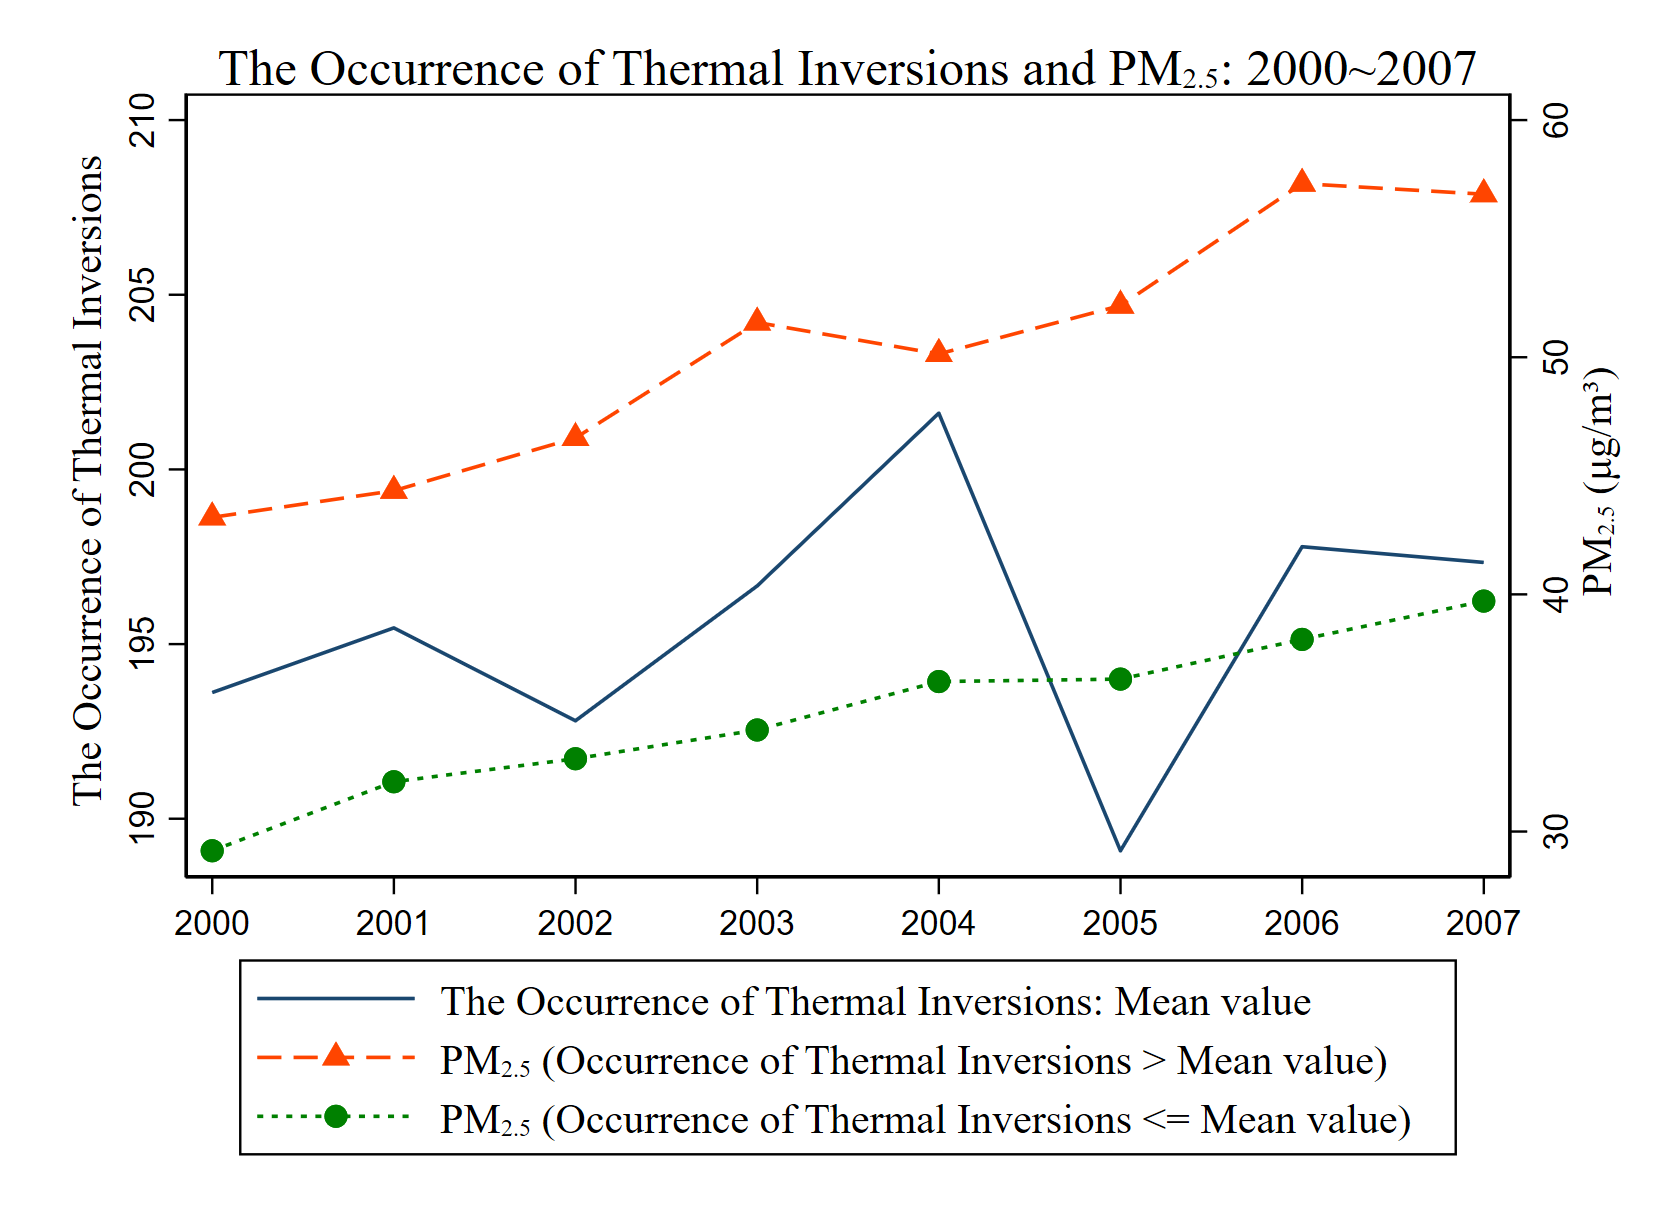
\includegraphics[height=.35\textheight,keepaspectratio]{TI_PM25_2.eps}
 %   \end{minipage}
    \small
    \caption*{Notes: The top panel plots the averages of PM2.5 of counties ranking in their averages of annual days of thermal inversions. The horizontal axis shows the quantiles of the counties' thermal-inversion distribution. Only counties within 10-90\% quantiles of the thermal-inversion distribution are presented.  
    The bottom panel shows the correlation between PM2.5 and thermal inversions. The green  dash line marked with dots plots the average annual occurrence in days of thermal inversions over counties from year 1998 to 2007. The red dash line marked with triangle plots the average annual PM2.5 of counties whose occurrence of thermal inversions is above the average level, and the blue dash line plots the average annual PM2.5 of counties whose occurrence of thermal inversions is below the average level.}
  \end{figure}


  \begin{figure}[H]\centering
    \caption{Average PM2.5 Concentrations of Counties in the Sample over 1998-2007 }\label{fig:3}
    \includegraphics[width=\textwidth]{PM98-07mean.eps}
  \end{figure}

\begin{figure}
\centering
\caption{Trends of Average PM2.5 and Exports}\label{fig:4}
\begin{subfigure}[b]{.75\textwidth}
\centering
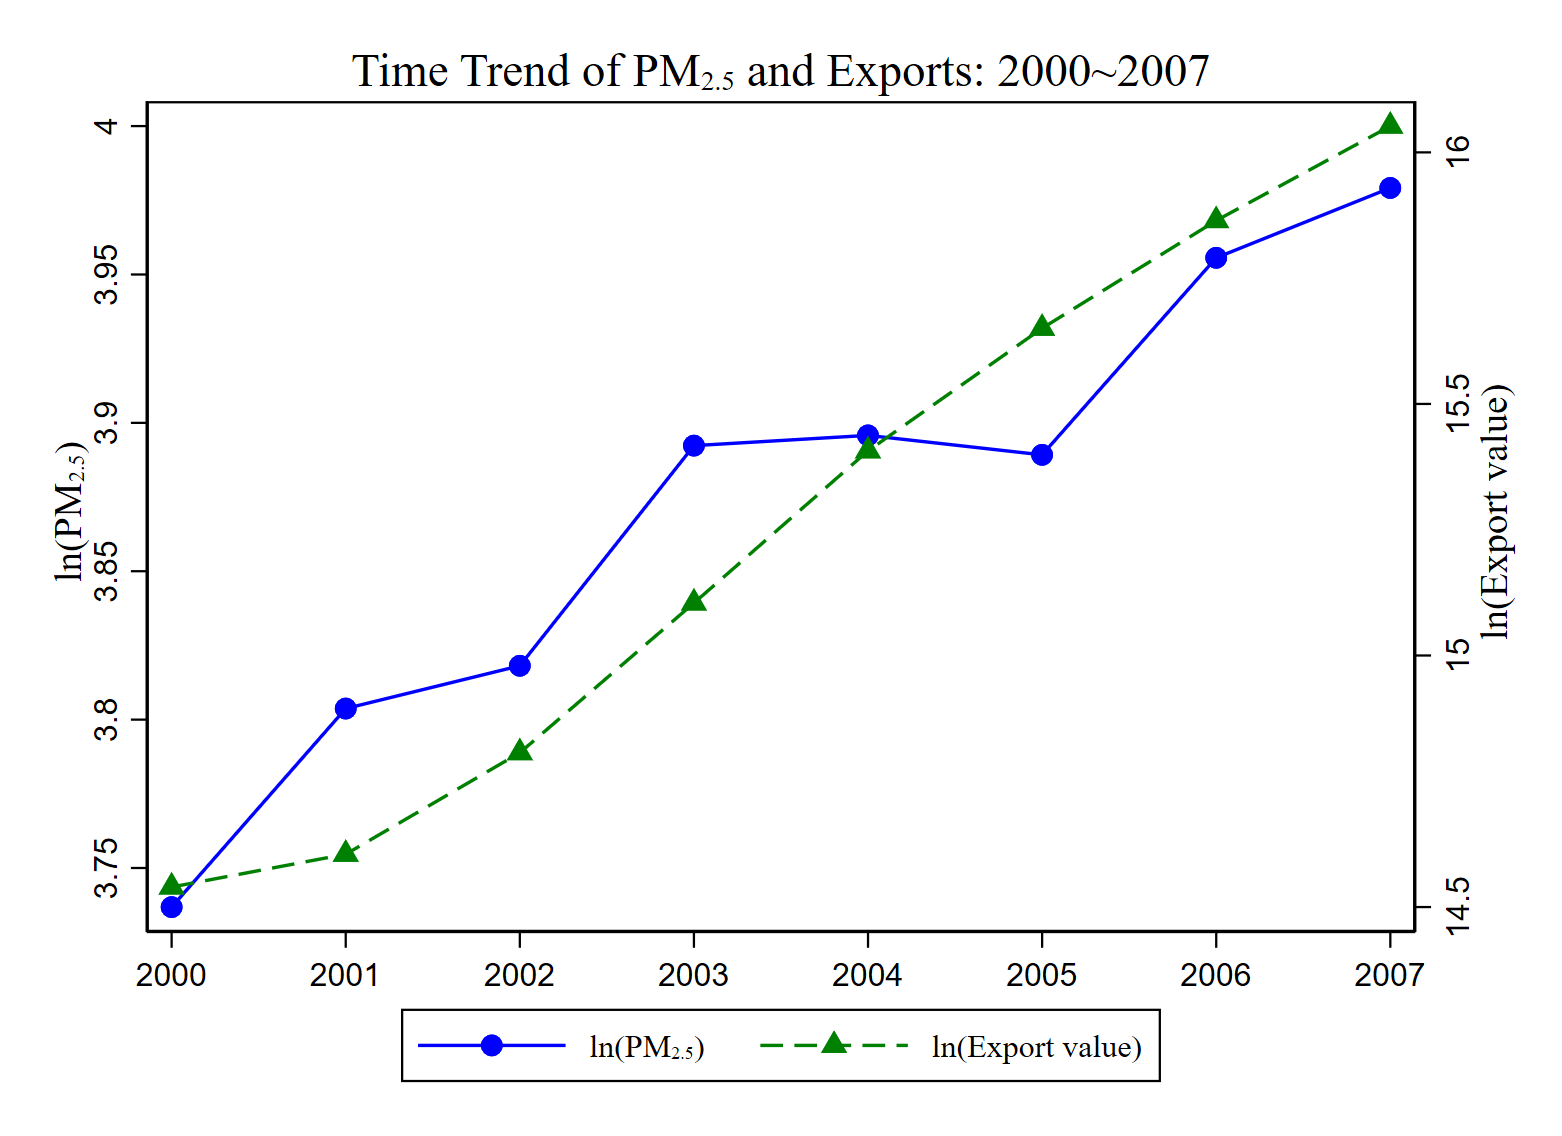
\includegraphics[width=\linewidth]{exp_pm25_trend.eps}
        \caption{}\label{fig:fig_a}
\end{subfigure}
%
\begin{subfigure}[b]{.75\textwidth}
\centering
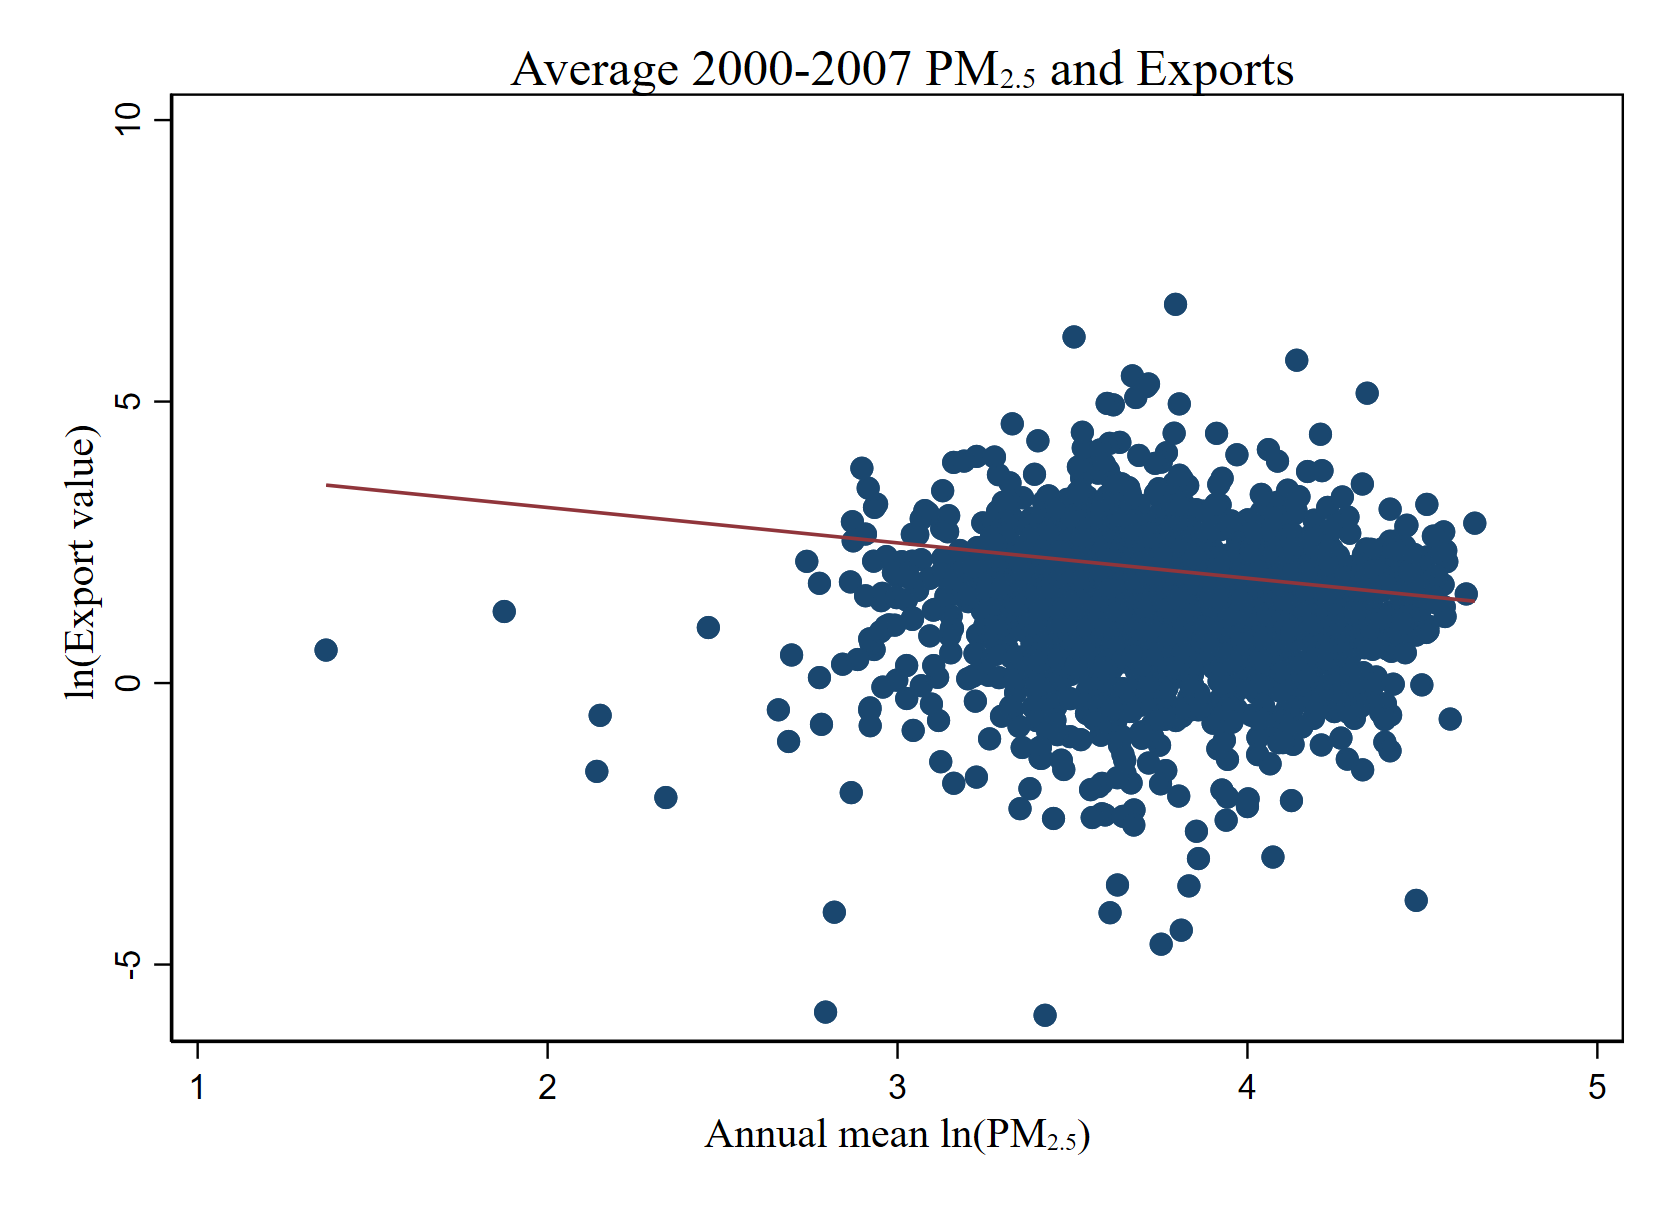
\includegraphics[width=\linewidth]{exp_pm25.eps}
\caption{}\label{fig:fig_b}
\end{subfigure}
\caption*{Notes: The top panel displays the trends of yearly averages of PM2.5 and exports of the sample counties from 2000 to 2007. The bottom panel displays the scatter of the county-level averages of PM2.5 and exports. The error terms of the fitted regression line are weighted by the number of firms in each county.}
\end{figure}

%   \begin{figure}[H]
%     \caption{}\label{fig:4}
%     \centering
%     \begin{minipage}[b]{0.8\textwidth}
%       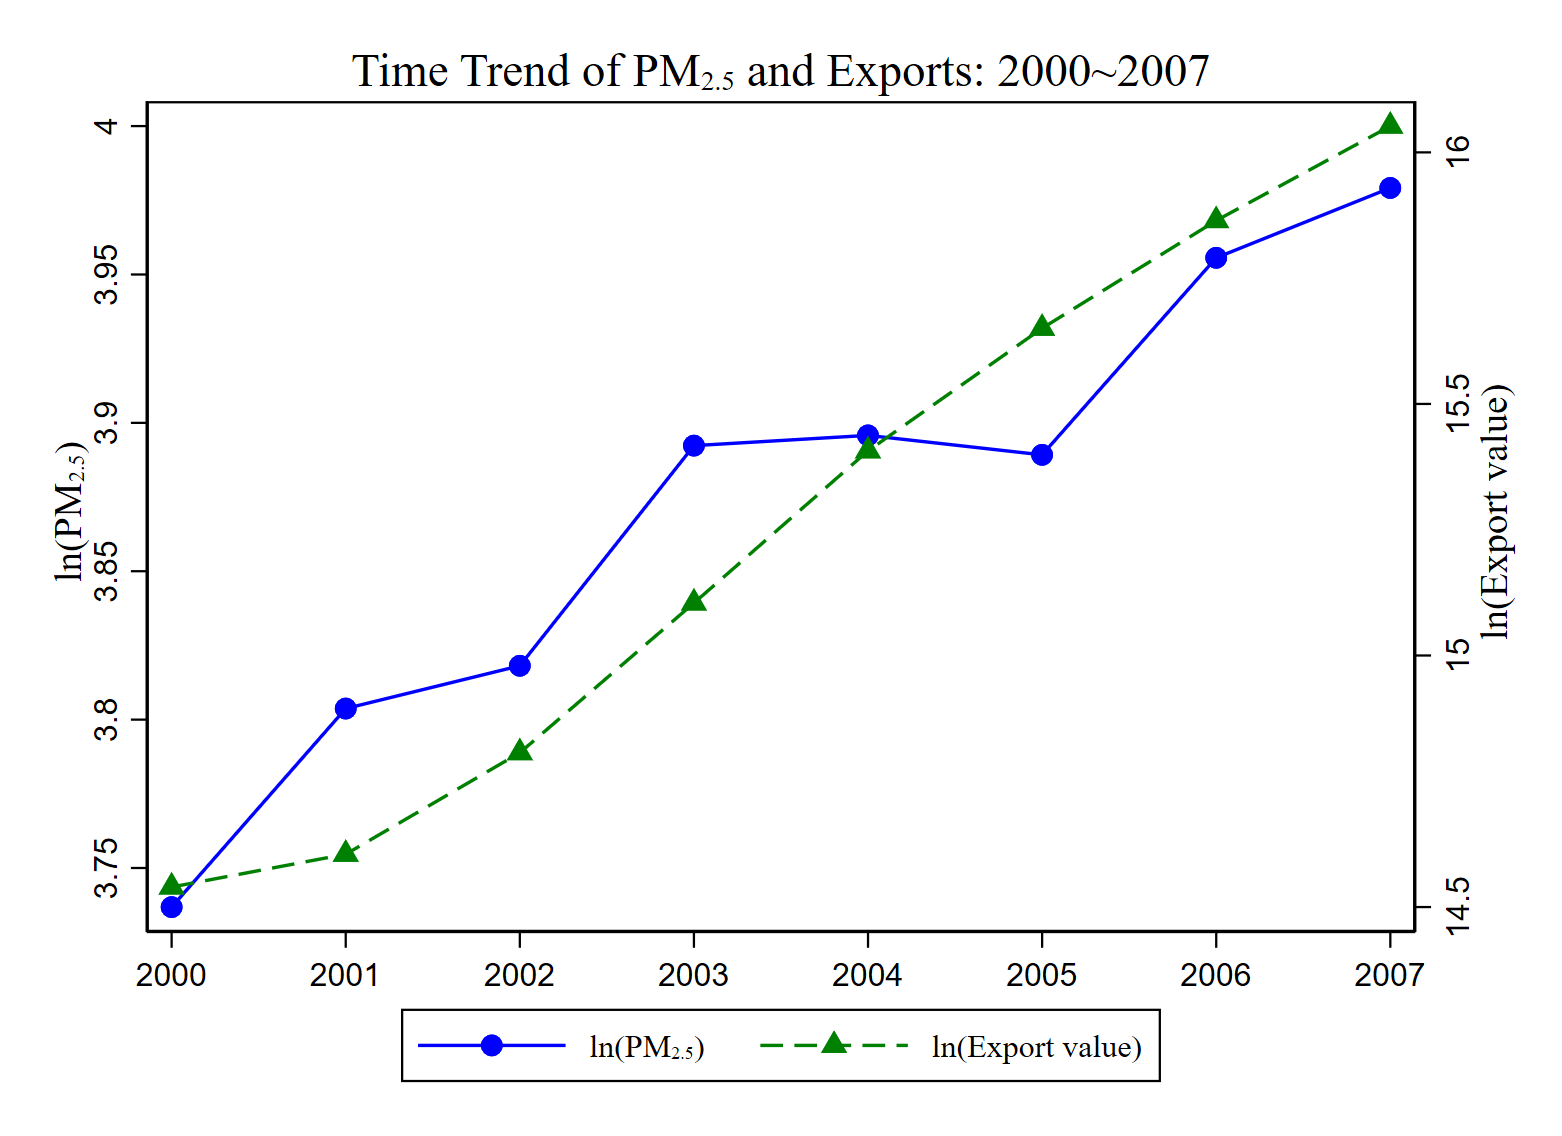
\includegraphics[width=\textwidth]{exp_pm25_trend.eps}
%     \end{minipage}
%     \begin{minipage}[b]{0.8\textwidth}
%       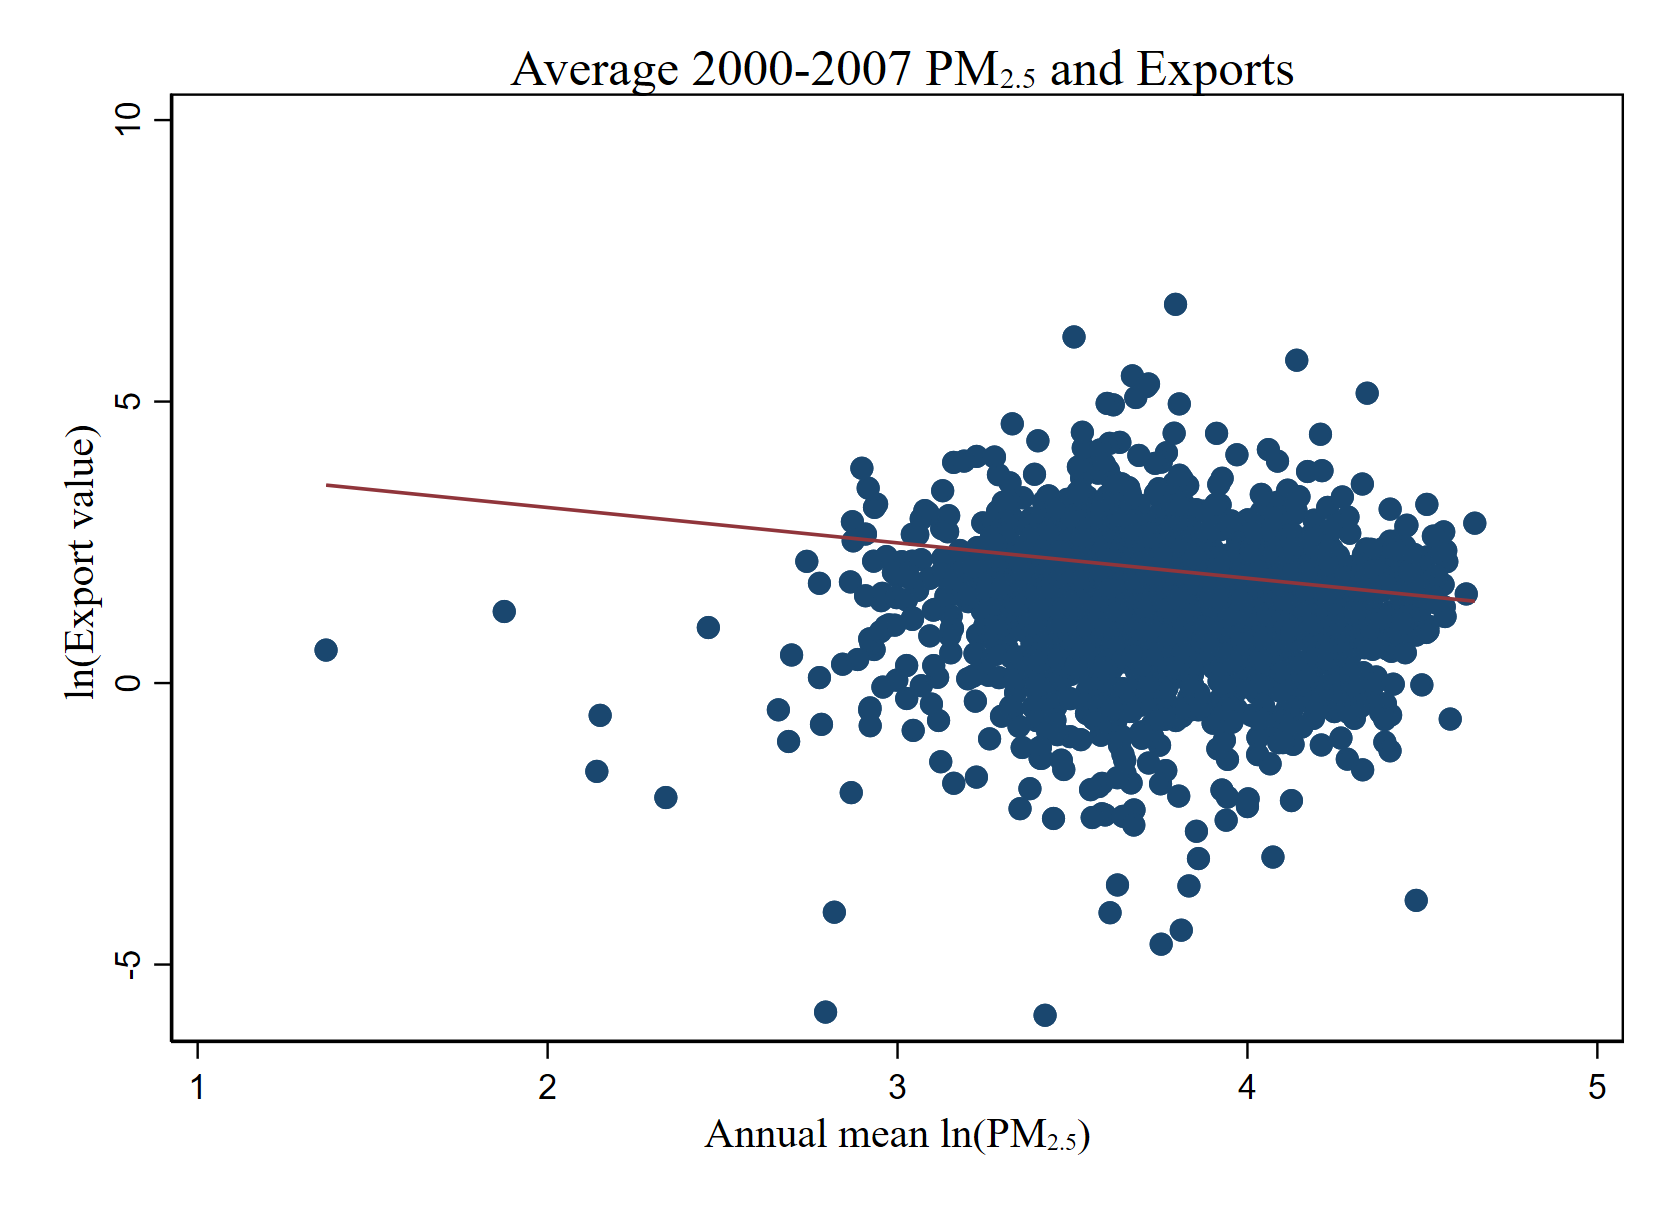
\includegraphics[width=\textwidth]{exp_pm25.eps}
%     \end{minipage}
%     \small
%     \caption*{Notes: The top panel displays the trend of yearly average PM2.5 and export from 2000 to 2007. In bottom panel, the export and PM2.5 is year-county observations. The average number of export firms is used as a weight to give more weights to counties with more exporting firms.}
%   \end{figure}


    \newpage
    % Make the "Part I" text invisible
    \renewcommand \thepart{}
    \renewcommand \partname{}
    \doparttoc % Tell to minitoc to generate a toc for the parts
    \faketableofcontents % Run a fake tableofcontents command for the partocs
    \appendix
    \addcontentsline{toc}{section}{Appendix} % Add the appendix text to the document TOC
    \setcounter{table}{0}
    \renewcommand{\thetable}{A\arabic{table}}
    \part{Appendix} % Start the appendix part
    \parttoc 
    \section{Robustness Check}
This section provides additional estimation results testing the robustness of our empirical analysis to the sample selection and model specifications.      
    \subsection{The effects of air pollution on intensive margin of exports}\label{sec:A.1}
     We extend our sample to include the exporting firms with intermittent positive export values to test the sensitivity of our estimation results to sample selection. As this sample includes all active exporting firms during the sample period, the estimation results reveals how the existing export values, or the intensive margin of export values, change in response to the changes in air pollution.  
     The estimation results are presented in Table~\ref{tab:A1}.
    \begin{table}[H]\centering
      \caption{The impact of air pollution on the intensive margin of export values}\label{tab:A1}
      \resizebox{\textwidth}{!}
      {
      \begin{tabular}{l*{6}{c}}
        \hline\hline
        &\multicolumn{1}{c}{(1)}&\multicolumn{1}{c}{(2)}&\multicolumn{1}{c}{(3)}&\multicolumn{1}{c}{(4)}&\multicolumn{1}{c}{(5)}&\multicolumn{1}{c}{(6)}\\
        Dep. var. &&&&\\ 
        $Log(Export)$ &&&&\\
        \hline
        $Log(PM_{2.5})$     & -1.3130***& -1.5411***&-1.5011***&-1.4976***&-1.5411**& -1.5411**\\
                                  &(0.4715)&(0.4715)  &(0.4572)  &(0.4567)& (0.7779) &(0.7199)\\
        log(Firm age)              &        &0.0304**  &0.0312**  &0.0299**&0.0304*&0.0304***\\
                                  &         &(0.0122) &(0.0122)  &(0.0122)&(0.0160)&(0.0110)\\
        log(Firm size)             &         &0.4321***&0.4963*** &0.6073***&0.4321***&0.4321***\\
                                  &         &(0.0085) &(0.0084)  &(0.0088)&(0.0134)&(0.0083)\\
        log(Firm capital)          &         &0.1609***&0.2026***& 0.1296***&0.1609***&0.1609***\\
                                  &         &(0.0055) &(0.0056) &(0.0055)&(0.0085)&(0.0056)\\
        $TFP_{LP}$                &         &0.1951***&         &        &0.1951***&0.1951***\\
                                  &         &(0.0045) &         &        &(0.0067)&(0.0047)\\
        $TFP_{OP}$                &         &          &0.1765***&&&\\
                                  &         &          &(0.0042)&&&\\
        \textit{Labor productivity} &      &           &&0.2068***&&\\
                                    &      &           &&(0.0046)&&\\
        \hline
        Cluster by firm  &Y&Y&Y&Y&&\\
        Cluster by county &&&&&Y&\\
        Cluster by county-year&&&&&&Y\\
        Firm FE &Y&Y&Y&Y&Y&Y\\
        Year FE &Y&Y&Y&Y&Y&Y\\
        Weather controls &Y&Y&Y&Y&Y&Y\\
        \hline
        Observations    &284,666&284,666&284,666  &284,666&284,666&284,666\\
        Firms           &68,105 &68,105 &68,105   &68,105&68,105&68,105\\
        KP F-statistic   &1080.50 &1081.47& 1081.78&1082.15&15.25&30.29\\
        Estimation      &TSLS&TSLS&TSLS&TSLS&TSLS&TSLS \\
        \hline\hline
      \end{tabular}
      }
      \begin{tablenotes}
        \item[*] \small Notes:  KP F-statistic is Kleibergen-Paap Wald rk F-statistic for weak identification test in the stage one estimation. We calculate 20 quantiles of the overall daily distribution of temperature. For each county-year observation in the data, we then calculate the share of days that fall into each of the 20 quantiles following \citep{deschenes2017defensive}. Weather controls include this 20-dimension vector of shares of days in the temperature distribution and the second-order polynomials of precipitation, humidity, wind speed, and sunshine duration. Standard errors are clustered at the firm level in Columns (1) - (4), at county level in Column (5), at the county-by-year level in Column (6), and are reported in parentheses. Statistical significance is denoted by: * p $<$ 0.1, ** p $<$ 0.05, *** p $<$ 0.01.
      \end{tablenotes}
      \end{table}
    
    \subsection{Robustness check on instrumental variable}
    In the main content, we measure TI by counting the yearly occurrence in days of reversal of the normal temperature behaviour between the lowest and the second lowest levels in the troposphere. TI between these two layers plays the most important role in trapping the air pollution. However, its effects could depend on temperature, humidity and other weather factors. These factors could make TI between other lays become more important in determining air pollution. 
    
    This section tests the robustness of our results to the other measures of TI and use them as IV for TSLS estimation. Specifically, we measure TI by counting the yearly occurrence in days of reversal of the normal temperature behaviour between the the lowest and the third lowest levels in the troposphere. The estimation results are presented in Table~\ref{tab:TI_alt}. The results suggest that all main conclusions remain, and our findings are robust to different measures of TI. 
    
    \begin{table}[H]\centering
      \caption{Robustness checks: alternative layers of inversions}\label{tab:TI_alt}
      \begin{tabular}{l*{4}{c}}
        \hline\hline
        &\multicolumn{1}{c}{(1)}&\multicolumn{1}{c}{(2)}&\multicolumn{1}{c}{(3)}&\multicolumn{1}{c}{(4)}\\
        Dep. var. $Log(Export)$  &&&&\\ 
        \hline
        $Log(PM_{2.5})$     &-3.9860***&-4.2872***&-4.2032***&-4.2702***\\
                            &(0.9545)&(0.9266)&(0.9260)&(0.9258)\\
        log(Productivity) &&0.2033***&0.1854***&0.2150***\\
                                  &&(0.0047)&(0.0044)&(0.0049)\\
        log(Firm age)  &&0.0615***&0.0634***&0.0606***\\
                      &&(0.0134)&(0.0134)&(0.0134)\\
        log(Firm size) &&0.4324***&0.4993***&0.6148***\\
                      &&(0.0089)&(0.0088)&(0.0092)\\
        log(Firm capital) &&0.1602***&0.2038***&0.1277***\\
                          &&(0.0059)&(0.0060)&(0.0059)\\
        \hline
        Firm FE &Y&Y&Y&Y\\
        Year FE &Y&Y&Y&Y\\
        Weather controls &Y&Y&Y&Y\\
        \hline
        Observations   &236,494&236,494&236,494&236,494\\
        Firms          &55,017 &55,017 &55,017&55,017\\
        KP F-statistic &360.60&356.77&357.22&356.82\\
        Estimation &TSLS&TSLS&TSLS&TSLS\\
        \hline\hline
      \end{tabular}

      \begin{tablenotes}
        \item[*] \small Notes: Columns (2), (3) and (4) report the results with productivity being measured by LP-method TFP, OP-method TFP and labor productivity, respectively. Results from TSLS estimation are reported. This sample consists of firms with positive exports between their first and last periods of exports during the sample period. We calculate 20 quantiles of the overall daily distribution of temperature. For each county-year observation in the data, we then calculate the share of days that fall into each of the 20 quantiles following \citep{deschenes2017defensive}. Weather controls include this 20-dimension vector of shares of days in the temperature distribution and the second-order polynomials of precipitation, humidity, wind speed, and sunshine duration. To control for potential auto-correlations of the error terms within firms, the standard errors are clustered by firm. Statistical significance is denoted by: * p $<$ 0.1, ** p $<$ 0.05, *** p $<$ 0.01.
      \end{tablenotes}
      \end{table}
      
      \subsection{Weighted measures of air pollution and thermal inversion}
      In this section, we use weighted measures of county-level air pollution and TI for our analysis. The measurement weight is the inverse squared distance between  the county centroid and the collection point of the pollution and TI data, the latitude-longitude grid cells in the DGG system, within the 200 kilometer radius of a county's centroid.  
      
      Table~\ref{tab:robust_weighted_measure} presents the results using the distance-weighted measures of air pollution and TI. All main conclusions remain, suggesting that our results are not sensitive to the degrees of importance of different data collection points in a county. 
      \begin{table}[H]\centering
        \caption{Results from TSLS Estimation Using Distance-weighted Measures of Air Pollution and TI}\label{tab:robust_weighted_measure}
        \resizebox{\textwidth}{!}
        {
        \begin{tabular}{l*{8}{c}}
          \hline\hline
          Dep. var.              &\multicolumn{4}{c}{\underline{Log(Export)}}&\multicolumn{2}{c}{\underline{Probability of exit}}&\multicolumn{2}{c}{\underline{Probability of entry}}\\
                              &\multicolumn{1}{c}{(1)}&\multicolumn{1}{c}{(2)}&\multicolumn{1}{c}{(3)}&\multicolumn{1}{c}{(4)}&\multicolumn{1}{c}{(5)}&\multicolumn{1}{c}{(6)}&\multicolumn{1}{c}{(7)}&\multicolumn{1}{c}{(8)}\\

          \hline
          $Log(PM_{2.5})$      & -1.2011**  & -1.3718***& -1.3567*** &-1.3245*** &0.1602***&0.1619***&-0.0513*** &-0.0650***\\
                               &  (0.5203)  & (0.5013) & (0.5020)  &  (0.5009)    &(0.0081) &(0.0082)&(0.0020)& (0.0020)      \\
    
          log(Productivity)    &             &0.2004***&0.1833***  & 0.2117***    &        &0.0002&   &0.0019***\\
                               &             &(0.0046)&(0.0044)   &  (0.0047)     &        &(0.0005)&&(0.0002)\\
          log(Firm age)        &             &0.0637***&0.0655***  & 0.0629***    &        &0.0157***&&-0.0143***\\
                               &              &(0.0133)&(0.0133)   & (0.0133)     &        &(0.0010)&&(0.0003)\\
          log(Firm size)       &             &0.4341***&0.5000***  & 0.6138***    &        &-0.0105***&&0.0131***\\
                               &              &(0.0088)&(0.0087)   &  (0.0091)    &        &(0.0006)&&(0.0003)\\
          log(Firm capital)    &             &0.1657***&0.2087***  & 0.1337***    &        &0.0070***&&0.0055***\\
                               &              &(0.0056)&(0.0058)   & (0.0057)     &        &(0.0005)&&(0.0002)\\
          \hline
          Firm FE          &Y&Y&Y&Y&&&&\\
          Year FE          &Y&Y&Y&Y&&&&\\
          Weather controls &Y&Y&Y&Y&Y&Y&Y&Y\\
          \hline
          Observations   &236,494&236,494&236,494&236,494 &222,716&222,716&773,050&773,050\\
          Firms          &55,017 &55,017&55,017 &55,017  & 71,615&71,615&264,218&264,218\\
          KP F-statistic &1299.62&1304.70&1304.08&1305.74&&&&\\
          Estimation &TSLS&TSLS&TSLS&TSLS&IV-Probit&IV-Probit&IV-Probit&IV-Probit\\
          \hline\hline
        \end{tabular}
        }
        \begin{tablenotes}
          \item[*] \small Notes: Columns (2), (6) and (8) report the results with productivity being measured by LP-method TFP; Column (3) and (4) reports the results with productivity being measured by OP-method TFP and labor productivity, respectively. This sample consists of firms with positive exports between their first and last periods of exports during the sample period. We calculate 20 quantiles of the overall daily distribution of temperature. For each county-year observation in the data, we then calculate the share of days that fall into each of the 20 quantiles following \citep{deschenes2017defensive}. Weather controls include this 20-dimension vector of shares of days in the temperature distribution and the second-order polynomials of precipitation, humidity, wind speed, and sunshine duration. To control for potential auto-correlations of the error terms within firms, the standard errors are clustered by firm. Statistical significance is denoted by: * p $<$ 0.1, ** p $<$ 0.05, *** p $<$ 0.01. 
        \end{tablenotes}
      \end{table}
\end{document}